% !TEX encoding = UTF-8 Unicode
%!TEX root = thesis.tex
% !TEX spellcheck = en-US
%%=========================================
\chapter[Method]{Method}\label{ch:Method}

Outlining the various choices, motivations, and approaches used during the current project, this chapter details our method for identifying three-dimensional hyperbolic LCSs. Starting out by summarizing the numerical treatment of system velocity fields and resulting strain characteristics, we describe methods for efficiently performing the necessary field interpolation and solving ODEs. The hyperbolic LCS existence criteria outlined in chapter \ref{ch:Theory} are then adapted as to facilitate numerical analysis. Prompted by these criteria, we then adapt the method of geodesic levelsets first described by \cite{GeodesicLevelSets} to compute LCS candidate manifolds. Two different approaches to adapting the method of geodesic levelsets are presented and compared with respect to accuracy, performance, and clarity. We finally devise a method for extracting hyperbolic LCSs from these candidate manifolds. 

\section{Tracer advection}\label{sec:tracer_advection}

Aiming to describe the overarching structures of complex flow systems in a finite-time interval, efforts of LCS identification are usually developed from flow maps. As discussed in section \ref{sec:TransportSystems}, the flow map $\vec{F}_{t_0}^t(\vec{x}_0)$ maps the initial position at $t_0$ of each particle in the system to its position at time $t$. In numerical analysis, a flow map is developed by advecting a set of particles in a velocity field  by use of an iterative ODE solver. The velocity field for a fluid flow system may for example be attained by use of the Navier-Stokes equations, or in principle --- if not necessarily in practice --- by direct measurements. Attainment of the velocity field is however beyond the scope of this investigation.

Forming the basis of all further analysis, the flow map $\vec{F}_{t_0}^t(\vec{x}_0)$ is computed for a regular grid of $N=N_xN_yN_z$ initial positions on and within the boundaries of the region of interest $U$. This is done by advecting tracer particles initially placed at the initial positions $\vec{x}_0$ in the governing velocity field. As outlined in section \ref{sec:FlowMapDynamics}, the flow map is developed in time while simultaneously solving the variational equation \eqref{eq:var_eq_2}, also providing us with the flow map Jacobian $\nabla\vec{F}_{t_0}^t(\vec{x}_0)$. This corresponds to simultaneously solving the set of $12$ coupled equations given by the Cartesian forms of equation \eqref{eq:var_eq_1} and equation \eqref{eq:var_eq_2}. We do this by use of the Dormand-Prince adaptive step method of orders $7$ and $8$. See sections \ref{sec:ODEs} and \ref{sec:automatic_step_control} for further details. 

Performing this computation is quite costly for large grids consisting of millions of tracers, requiring the use of parallel computing. As each tracer particle is independent of the remaining grid, this is easily done, for example by use of MPI and the \textit{mpi4py} Python library. Specifically, the tracer particles are distributed evenly among all available processing cores, where the variational equations are solved for the considered time interval. Finally, the results are passed to the main process for further analysis.

The system of $12$ coupled equations carries an added computational load compared to simply advecting the tracer particles. Consider however that the most notable alternative approach, proposed by \cite{Haller12}, for computing the flow map Jacobian entails advecting an additional auxiliary grid of six tracers per main grid tracer. The number of equations needed to be solved per time step is therefore $21N$ for \cite{Haller12}'s approach, and only $12N$ for the current one. While adding some complexity to the computation, the method of variational equations is therefore preferred both due to its superior accuracy \citep{Oettinger} and efficiency.

%%=========================================
\subsection{Implementation of automatic step control}\label{sec:automatic_step_control}

The flow map advection described in section \ref{sec:tracer_advection} and the point search trajectories to be described in section \ref{sec:trajectories} are both computed by use of the Dormand-Prince method of orders $7$ and $8$. As noted in section \ref{sec:adaptive_step}, this method uses the difference between a $7$\ts{th}- and an $8$\ts{th}-order Runge-Kutta solution, $\vec {\bar{x}}_{n+1}-\vec{\widehat{x}}_{n+1}$, to automatically control step length. Here, $\vec{\widehat{x}}_{n+1}$ is the $7$\ts{th}-order $(n+1)$\ts{th} Runge-Kutta ODE solution step, while $\vec{\bar{x}}_{n+1}$ is the corresponding $8$\ts{th}-order solution. Inspired by \cite{SolvingODEs}, we control the step length by limiting the componentwise error according to

\begin{equation}
\left|\bar{x}_i-\widehat{x}_i\right| \leq sc_i,
\end{equation}

\noindent where

\begin{equation}
sc_i = \text{Atol}_i + \text{max}\left(\left|\bar{x}_i\right|,\left|\widehat{x}_i\right|\right)\cdot \text{Rtol}_i,
\end{equation}

\noindent is our componentwise error limit and the parameters

\begin{equation}
\text{Atol}_i = \text{Rtol}_i = 10^{-7}
\end{equation}

\noindent are used consistently. This allows us to define our error measure

\begin{equation}\label{eq:error}
err = \sqrt{\frac{1}{\mathcal{N}}\sum_{i=1}^{\mathcal{N}}\left(\frac{\bar{x}_{n+1,i}-\widehat{x}_{n+1,i}}{sc_i}\right)^2},
\end{equation}

\noindent (where $\mathcal{N}$ is the number of simultaneously computed variables) and use $\epsilon_{\text{tol}}=1$ in equation \eqref{eq:step_condition}, yielding the step acceptance criterion

\begin{equation}\label{eq:compare_to_unity}
err \leq 1.
\end{equation} 

\noindent Finally, the ideal step length $\Delta t_{\text{opt}}$ is determined by inserting $\epsilon_{\text{tol}}=1$ into equation \eqref{eq:dt_new}, yielding

\begin{equation}
\Delta t_{\text{opt}} = \Delta t\left(\frac{1}{err}\right)^\frac{1}{p+1},
\end{equation}

\noindent where $p=7$ is the order of the least accurate Runge-Kutta method. 

Now, all steps that satisfy equation \eqref{eq:compare_to_unity} are accepted,  while steps that do not satisfy \eqref{eq:compare_to_unity} are rejected. That is, as long as equation \eqref{eq:compare_to_unity} is satisfied, we adopt the approximation $\vec{x}_{n+1} = \vec{\bar{x}}_{n+1}$ for next next time step $t_{n+1}=t_n+\Delta t$. The new step lengths are computed according to

\begin{equation}
	\Delta t_{\text{new}} = 
	\begin{cases}
    \text{min}\left(\text{fac}_{\text{max}}\cdot \Delta t, \text{fac}\cdot \Delta t_{\text{opt}}\right) & \text{if step is accepted} \\
    \text{fac}\cdot \Delta t_{\text{opt}} & \text{if step is rejected}.
    \end{cases}
\end{equation}

\noindent Here, $\text{fac}=0.8$ and $\text{fac}_{\text{max}}=2.0$ are numerical safety factors, preventing excessive increases in step length and increasing the likelihood of the next step being accepted.

Note that while each coordinate in the three-dimensional system is managed independently, the corresponding time step lengths must be identical, prompting us to --- for each step --- apply the largest $\Delta t_{\text{new}}$ to all coordinate ODEs.

Also note that the Dormand-Prince ODE solver, used to compute manifold points (see section \ref{sec:trajectories}), was implemented in Cython as to improve performance. This was done in order to retain the ease of development, as well as comprehensibility, of Python, while maximizing performance in computationally heavy operations.



%%=========================================
\subsection{Velocity field interpolation}\label{sec:velocity_interpolation}

Unlike investigations of three-dimensional analytical velocity fields, analysis of time-varying gridded model data in three dimensions requires the use of a quadrivariate interpolator. Specifically, this is needed to compute the accompanying flow map. Considering each velocity field component separately, they are interpolated in time as well as the three spatial coordinates. As suggested by \cite{OptimalInterpolation}, this was done by use of cubic B-splines (see section \ref{sec:SplineInterpolation}). Several multidimensional B-spline interpolation libraries are currently available. Choosing the \textit{Bspline-Fortran} library for its performance and comprehensive documentation \citep{Williams18}, quadrivariate velocity field interpolation was carried out using the \texttt{bspline\_}\texttt{4d} derived type. This Fortran tool was made available in Python through the Fortran standard C interoperability. By writing a C++ wrapper class, the solver was made available in Python via Cython. Note that memory duplication was minimized by use of the Fortran reference-based subroutine call structures, as well as pointers at the C-level. This is critical, as large memory requirements could limit the efficiency of parallelization. Specifically, memory-intensive tasks could require us to use several computing cores per parallel process in order to pool memory, dramatically increasing resource usage.

%%=========================================
\section{Computing Cauchy-Green strain tensor eigenvalue and eigenvector fields}\label{sec:Cauchy-Green_eigen}

Enabling further deformation analysis and identification of LCSs, the Cauchy-Green eigenvectors $\bm{\xi}_i(\vec{x}_0)$ and eigenvalues $\lambda_i(\vec{x}_0)$ were computed at the tracer initial position grid by use of singular-value decomposition. As outlined in section \ref{sec:SVD}, this allows us to implicitly determine $\bm{\xi}_i(\vec{x}_0)$ and $\lambda_i(\vec{x}_0)$ without having to compute the Cauchy-Green strain tensor $\vec{C}_{t_0}^{t}(\vec{x}_0)$. In this way, we limit the error introduced by floating point arithmetic \citep{Watkins05}. Singular-value decomposition algorithms are widely available, for example in the \textit{NumPy} library \citep{numpy}.

%%=========================================
\subsection{Cauchy-Green eigenvalue field interpolation}\label{sec:eigenvalue_interpolation}

Identifying LCSs in the previously described discrete eigenvector and eigenvalue fields necessitates use of interpolation. That is, as we analyze off-grid points in $U$ with regard to the existence conditions \ref{eq:ExistenceConditions}, we will need interpolated values for the eigenvalue fields $\lambda_2(\vec{x}_0)$ and $\lambda_3(\vec{x}_0)$.

These eigenvalue fields were interpolated by use of cubic trivariate B-splines, ensuring continuous first and second derivatives. Note that this use of cubic B-splines, ensuring continuous second derivatives, is necessary for evaluating the Hessian of $\lambda_3(\vec{x}_0)$ in existence condition 2 (see equation \eqref{eq:ExistenceConditions}). This was done by use of the \texttt{bspline\_}\texttt{3d} derived type from the \textit{Bspline-Fortran} library. Like previously described in section \ref{sec:velocity_interpolation}, this method was made available in Python by use of Cython.

%%=========================================
\subsection{Cauchy-Green eigenvector field interpolation}\label{sec:eigenvector_interpolation}

Accompanying the interpolated eigenvalue fields, LCSs identification requires a continuous $\bm{\xi}_3$-field. That is, as we construct surfaces according to condition $3$ in equation \eqref{eq:ExistenceConditions}, it becomes necessary to evaluate the $\bm{\xi}_3$-field between grid points.

While ultimately treated in the same way as the eigenvalue field --- using the \texttt{bspline\_}\texttt{3d} derived type from the \textit{Bspline-Fortran} library --- the eigenvector field requires some additional treatment. Specifically, as the stretching along $\bm{\xi}_i(\vec{x}_0)$ and $-\bm{\xi}_i(\vec{x}_0)$ is the same, there is no \textit{a} \textit{priori} reason to assume the singular-value decomposition consistently chose any specific orientation. As our cubic B-spline interpolation routine imposes continuity of the eigenvector components, it is critical that the underlying field exhibits this trait. Otherwise, it is likely that the resulting B-spline interpolation will be inaccurate. Continuity of eigenvector components was ensured by use of a three-dimensional local orientation correction scheme, adapted from the two-dimensional case outlined by \cite{LCStool}.

Local orientation continuity is ensured by considering the set of $64$ nearest neighbor grid points of the considered coordinate. Note that $4^3=64$ is the smallest number of nearest neighbor grid eigenvector values required to compute a local trivariate cubic spline interpolation. Assuming that the extent of this neighborhood is small compared to the scale over which significant orientational changes may occur in the eigenvector field, we ensure that no input grid vectors are oriented in opposing directions. This is done by selecting the eigenvector of a neighborhood corner as a reference direction. All remaining grid point eigenvectors are then compared to this reference direction by means of computing their inner product. Whenever this inner product evaluates to less than zero, the current grid point eigenvector is reversed. That is, we exchange $\bm{\xi}_3(\vec{x}_0)$ for $-\bm{\xi}_3(\vec{x}_0)$. The two-dimensional equivalent of this algorithm is demonstrated in figure \ref{fig:local_orientation_correction}. Note that while unsuited for representation in a two-dimensional figure, the three-dimensional scheme remains completely analogous. 

Following this local orientation correction, the neighborhood grid is passed to the \textit{Bspline-Fortran} interpolator method. The three-component output is finally normalized, conforming with the convention of normalized eigenvectors. 

%%=========================================
\section{Limit search to LCS existence subdomain}\label{sec:AB_subdomain}

As previously discussed in section \ref{sec:LCS_id}, three-dimensional hyperbolic LCSs may be identified as material surfaces forming local repulsion maxima. In order to limit the search for LCSs to the regions of the domain in which such maxima may exist, a subdomain of $U$ is defined as the set of points where conditions $1$, $2$ and $4$, given by equation \eqref{eq:ExistenceConditions}, hold. Here, condition 1 establishes that a direction of maximum repulsion exists, while condition 2 excludes all regions where no local maximum of $\lambda_3$ may occur. Finally, compliance with condition $4$ ensures that any given point $\vec{x}_0$ is a local maximum of $\lambda_3$ along the direction defined by $\bm{\xi}_3(\vec{x}_0)$. \cite{Haller12} note that condition $2$ may be made more appropriate for numerical analysis by also allowing for equality with zero. Moreover, compliance with condition $4$ may be checked by comparing $\lambda_3(\vec{x}_0)$ to $\lambda_3(\vec{x}_0+\epsilon\bm{\xi}_3(\vec{x}_0))$ and $\lambda_3(\vec{x}_0-\epsilon\bm{\xi}_3(\vec{x}_0))$, where $\epsilon$ is some appropriately chosen scalar. The resulting conditions used to obtain an ``ABD subdomain'' $U_{\text{ABD}}$ are

\begin{equation}\label{eq:LCS_condition_A}
	\text{(A)} \quad \lambda_2(\vec{x}_0) \neq \lambda_3(\vec{x}_0),\quad \lambda_3(\vec{x}_0) > 1,
\end{equation} 

\begin{equation}\label{eq:LCS_condition_B}
	\text{(B)} \quad \left\langle \bm{\xi}_3(\vec{x}_0), H_{\lambda_3}(\vec{x}_0)\bm{\xi}_3(\vec{x}_0)\right\rangle \leq 0,
\end{equation}

\begin{equation}\label{eq:LCS_condition_D}
	\text{(D)} \quad \lambda_3(\vec{x}_0) > \text{max}(\lambda_3(\vec{x}_0 - \epsilon\bm{\xi}_3(\vec{x}_0)), \lambda_3(\vec{x}_0 + \epsilon\bm{\xi}_3(\vec{x}_0))),
\end{equation}


\noindent where $H_{\lambda_3}(\vec{x}_0)$ is the Hessian matrix (see equation \eqref{eq:Hessian}) of the largest Cauchy-Green eigenvalue. $H_{\lambda_3}(\vec{x}_0)$ was computed by taking the partial derivatives of the cubic spline interpolation of $\lambda_3(\vec{x}_0)$.

\begin{figure}[h!] 
\centering
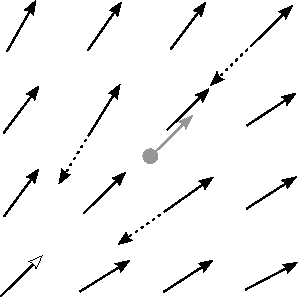
\includegraphics[width=70mm]{fig/orientation_correction.pdf}
\caption{Visualization of the chosen local orientation correction scheme in two dimensions. Allowing for cubic interpolation, the $4^2=16$ nearest neighbor eigenvector grid points of the evaluated point (in gray) are extracted and corrected using the lower left corner eigenvector (no arrow fill) as a reference. Considering each extracted vector, its inner product with the lower left corner eigenvector is evaluated. If this inner product evaluates to less than zero, the eigenvector is turned $180^{\circ}$ before passing to the interpolation routine. Note the dashed arrows indicating original eigenvector orientations where corrections have been performed. The resulting interpolated vector is presented in gray. This algorithm is generalized to three dimensions by using a grid of $4^3=64$ nearest neighbor eigenvectors.}\label{fig:local_orientation_correction}
\end{figure}

Subdomains $U_{\text{ABD}}$ obtained by applying conditions A, B, and D to the ABC flow test cases, as well as the fjord gridded model data set, described in sections \ref{sec:steady_abc_flow}-\ref{sec:fjord}, are presented in figures \ref{fig:time_indep_ABD}, \ref{fig:time_dep_ABD}, and \ref{fig:fjord_ABD_domain}.

%%=========================================
\section{Computing manifolds in Cauchy-Green eigenvector field by use of geodesic levelsets}\label{sec:GLS_intro}

As shown by \cite{Oettinger} and described in section \ref{sec:Oettinger}, hyperbolic LCSs in three-dimensional systems are invariant manifolds of the autonomous dynamical system described by equation \eqref{eq:hyperbolic_autonomous_dynamical_system}. This suggests an approach to three-dimensional repelling LCS identification centered around computing these manifolds, producing surfaces that satisfy condition 3 in \eqref{eq:ExistenceConditions}, alternatively expressed as

\begin{equation}\label{eq:LCS_condition_C}
	\text{(C)} \quad \mathcal{M}(\vec{x}_0,t_0) \parallel a\bm{\xi}_1(\vec{x}_0) + b\bm{\xi}_2(\vec{x}_0),
\end{equation}

\noindent where $a$ and $b$ are scalars. In other words, the manifold $\mathcal{M}$ is at any point $\vec{x}_0$ tangent to the plane spanned by the vectors $\bm{\xi}_1(\vec{x}_0)$ and $\bm{\xi}_2(\vec{x}_0)$. As already noted in section \ref{sec:LCS_id}, this is equivalent to $\mathcal{M}$ being perpendicular to $\bm{\xi}_3(\vec{x}_0)$ at all points. Also accounting for conditions A, B and D, presented in equations \eqref{eq:LCS_condition_A}, \eqref{eq:LCS_condition_B} and \eqref{eq:LCS_condition_D}, the locally most repelling surfaces are identified as hyperbolic LCSs.

As noted by \cite{Survey}, computing accurate multidimensional invariant manifolds is challenging, necessitating dedicated algorithms. Among other alternatives, \cite{Survey} suggest approximation by geodesic levelsets, originally described by \cite{GeodesicLevelSets}. Although initially intended for investigating manifolds described by functions of the form $\vec{x}'=\vec{f}(\vec{x})$, the method of geodesic levelsets may reasonably be adapted to identify manifolds defined by equation \eqref{eq:hyperbolic_autonomous_dynamical_system}. This method is based on computing successive sets of points forming topological circles, each point computed by developing a trajectory in the underlying direction field from the preceding levelset. Points are then inserted or removed as to keep the level of mesh detail consistent. The result is a mesh $M$ comprising radial strands of points along the invariant manifold, emanating from the initial position from which the manifold is developed. Some of the main terminology used to describe the method of geodesic levelsets is illustrated in figure \ref{fig:terminology}.

\begin{figure}[h!] 
\centering
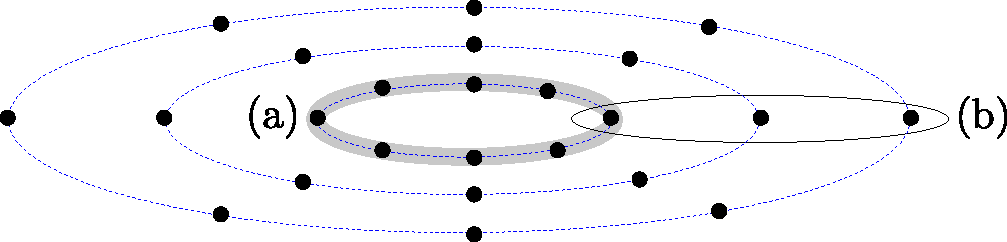
\includegraphics{fig/terminology.pdf}
\caption{Illustration of some of the main terminology used to describe the method of geodesic levelsets. (a) The set of mesh points covered by the shaded area form a geodesic levelset $M_i$. The corresponding dashed line is referred to as a topological circle $C_i$. (b) The outlined set of points emanating radially outwards is referred to as a point strand.}\label{fig:terminology}
\end{figure}

%%=========================================
\subsection{Selecting initial positions and computing subsequent mesh points}\label{sec:GLS_overview}

Having identified an initial position $\vec{r}_0$ in the target invariant manifold $\mathcal{M}$ described by equation \eqref{eq:hyperbolic_autonomous_dynamical_system}, a set of points are selected forming a small circle of radius $r_{\text{init}}$ centered at $\vec{r}_0$ in the plane spanned by $\bm{\xi}_1(\vec{r}_0)$ and $\bm{\xi}_2(\vec{r}_0)$. This is shown in figure \ref{fig:GeodesicLevelSet_first}. The selected points form the initial levelset $M_1$, which is subsequently interpolated as to form a continuous circle $C_1$. This was carried out by use of a cubic spline interpolation scheme. A more detailed description of this topological circle interpolation scheme may be found in section \ref{sec:topological_circles}.

\begin{figure}[h!] 
\centering
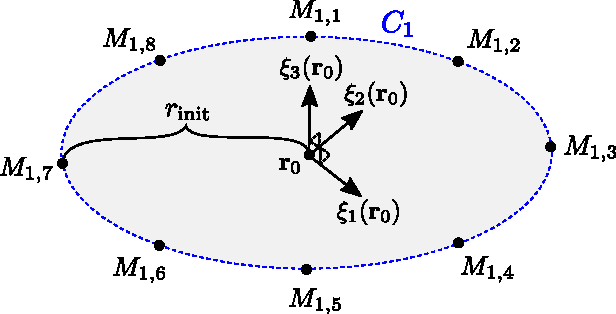
\includegraphics{fig/GeodesicLevelSet_first_2.pdf}
\caption{The initial levelset $M_1$ approximating a circle of radius $r_{\text{init}}$ around the initial position $\vec{r}_0$. The points $M_{1,j}$ are computed as various linear combinations of $\bm{\xi}_1(\vec{r}_0)$ and $\bm{\xi}_2(\vec{r}_0)$ added to the initial position $\vec{r}_0$. Choosing a sufficiently small radius $r_{\text{init}}$ and noting that as both $\bm{\xi}_1(\vec{r}_0)$ and $\bm{\xi}_2(\vec{r}_0)$ are perpendicular to $\bm{\xi}_3(\vec{r}_0)$, we assume that the set of points $\{M_{1,j}\}$ are all very close to the target manifold $\mathcal{M}$. The dashed topological circle $C_1$, approximated by interpolation of $M_1$, (see section \ref{sec:topological_circles}) is highlighted in blue.}\label{fig:GeodesicLevelSet_first}
\end{figure}

Each point in the first levelset $M_1$ is then used to compute a point in the subsequent levelset $M_{2}$. In the same way, all subsequent levelsets $M_{i+1}$ are initially computed starting with the prior levelset $M_i$. For the sake of brevity and intuitiveness in the coming discussion, we here denote the starting points in $M_i$ ,and new points in $M_{i+1}$, ancestor and descendant points, respectively. Moreover, the set of points consisting of an initial levelset point $M_{1,j}$ and and all its descendants $\{M_{i,j}\}_{i=2}^{m}$, where $m$ is the total number of levelsets, are referred to as a point strand. Here, point $j$ in levelset $i$ is denoted $M_{i,j}$. This is illustrated in figure \ref{fig:terminology}. %Finally, we drop the dependence of the Cauchy-Green eigenvectors on the initial position grid $\vec{x}_0$ in our notation, allowing us track these quantities in space.

In order to identify a new mesh point, consider the $j$\ts{th} point $M_{i,j}$ in the $i$\ts{th} levelset $M_i$. We search for a new point from the target manifold $\mathcal{M}$ in the half-plane $\mathcal{F}_r$ through $M_{i,j}$. This half-plane is orthogonal to $C_i$ at $M_{i,j}$ and stretches outwards, as defined by the vector $M_{i,j}-M_{i-1,j}$. As may be seen in figure \ref{fig:GeodesicLevelSet_br}, this restricts us to searching for points in the outward radial direction, while allowing for local curvature in the underlying manifold. \cite{Survey} suggest computing the normalized half-plane defining tangent vector at $M_{i,j}$ as

\begin{equation}\label{eq:surveyT}
\vec{T}(M_{i,j})=\frac{M_{i,j+1}-M_{i,j-1}}{\left|M_{i,j+1}-M_{i,j-1}\right|}.
\end{equation}

\noindent However, in practice, it was found that simply inheriting the tangent vector from $M_{1,j}$ yielded smoother manifolds that are less exposed to accumulation of numerical noise. That is, we define the initial normalized tangent vector according to

\begin{equation}\label{eq:ourT}
\vec{T}_j = \vec{T}(M_{1,j}) = \frac{\bm{\xi}_3(M_{1,j}) \times \left(M_{1,j}-\vec{r}_0\right)}{\left| \bm{\xi}_3(M_{1,j}) \times \left(M_{1,j}-\vec{r}_0\right)\right|},
\end{equation}

\noindent subsequently passing it on to all following points along the same strand. 



%\begin{figure}[h!] 
%\centering
%\includegraphics{fig/GeodesicLevelSet_Fr_2.pdf}
%\caption{PLACEHOLDER}\label{fig:GeodesicLevelSet_Fr}
%\end{figure}

We start the search for a new point $M_{i+1,j}$ within the target half-plane $\mathcal{F}_r$ by defining a position ``guess'' $\vec{r}_{\text{aim}}$, presumed to be close to the intersection of $\mathcal{M}$ with $\mathcal{F}_r$. In order to choose $\vec{r}_{\text{aim}}$, we begin by computing a single $4$\ts{th}-order Runge-Kutta step of length $\Delta_i$ from $M_{i,j}$. This is done by computing the cross product of the normalized tangent vector $\vec{T}$  and the underlying $\bm{\xi}_3$-field (see section \ref{sec:force_radially_outward} for details). Here, $\Delta_i$ is the prescribed inter-levelset step length, detailed in section \ref{sec:step_management}. %Finally, $\vec{r}_{\text{aim}}$ is determined by projecting the resulting position into the plane $\mathcal{F}_r$.

We find the point $M_{i+1,j}$ by computing trajectories along linear combinations of $\bm{\xi}_1(\vec{r})$ and $\bm{\xi}_2(\vec{r})$ from the prior topological circle $C_i$, aimed at $\vec{r}_{\text{aim}}$. A point along one of these trajectories is accepted as $M_{i+1,j}$ if it is both found to be within $\mathcal{F}_r$ and appropriately distanced from $M_{i,j}$. That is,

\begin{equation}\label{eq:within_dist_tol}
\left| \left| M_{i+1,j} - M_{i,j} \right| - \Delta_i \right| < \Gamma_{\Delta}\Delta_i
\end{equation}

\noindent is satisfied, where $\Gamma_{\Delta}$ is an inter-levelset separation tolerance factor. Moreover, sufficient proximity to $\mathcal{F}_r$ is defined as satisfying


\begin{equation}\label{eq:in_plane}
\frac{\vec{r} - M_{i,j}}{\left|\vec{r} - M_{i,j}\right|} \cdot \vec{T}_j< \Gamma_{\mathcal{F}_r},
\end{equation}

\noindent where $\vec{r}$ is the current trajectory position and $\Gamma_{\mathcal{F}_r}$ is some scalar tolerance parameter. Note that as no given trajectory is certain to produce an acceptable point, this process may have to be repeated for several initial positions on $C_i$. This trial and error process is outlined in section \ref{sec:trajectories}. Also notice that by construction, $M_{i+1,j}$ may only be situated on --- or very close to --- the half-circle within $\mathcal{F}_r$, centered at $M_{i,j}$, of radius $\Delta_i$. Refer to figure \ref{fig:GeodesicLevelSet_br} for a visual representation of this approach. 

\begin{figure}[h!] 
\centering
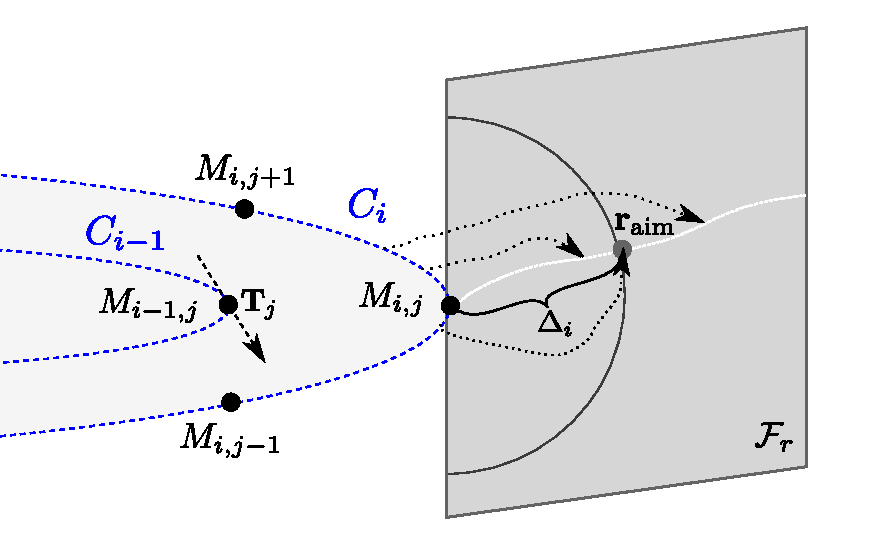
\includegraphics{fig/GeodesicLevelSet_br_2.pdf}
\caption{Computing a new mesh point $M_{i+1,j}$ within the half-plane $\mathcal{F}_r$. Using the inherited and normalized tangent vector $\vec{T}_j$ to define $\mathcal{F}_r$, the aim point $\vec{r}_{\text{aim}}$ is determined by taking a single $4$\ts{th}-order Runge-Kutta step of length $\Delta_i$ within $\mathcal{F}_r$. This $4$\ts{th}-order Runge-Kutta step is computed using the cross products of $\vec{T}_j$ and $\bm{\xi}_3(\vec{r})$, oriented along the vector $M_{i,j}-M_{i-1,j}$, where $\vec{r}$ is the current trajectory position. The trajectories from $C_i$ (black dashed curves) are then computed by projecting the vector $\vec{r}_{\text{aim}}-\vec{r}$ into the local plane characterized by orthogonality to $\bm{\xi}_3(\vec{r})$ (see section \ref{sec:trajectories}). These trajectories are terminated whenever they reach $\mathcal{F}_r$, as defined by equation \eqref{eq:in_plane}. If the concluding point of the trajectory $\vec{r}_{\text{end}}$ is approximately $\Delta_i$ away from $M_{i,j}$ (see equation \eqref{eq:within_dist_tol}), it is accepted as $M_{i+1,j}$. Otherwise, a new trajectory is computed from a different initial position on $C_i$. This choice of initial positions is outlined in section \ref{sec:trajectories}. The white dashed line represents the intersection of the target manifold $\mathcal{M}$ with the half-plane $\mathcal{F}_r$. Note that imposing the inter-levelset step length $\Delta_i$ ensures that the selected point is located at the displayed half-circle in the half-plane $\mathcal{F}_r$.}\label{fig:GeodesicLevelSet_br}
\end{figure}

%Also note the half-circle in $\mathcal{F}_r$ consisting of all possible positions $M_{i+1,j}$ could take.

%%=========================================
\subsection{Constructing topological circles from geodesic levelsets}\label{sec:topological_circles}

Providing an approximation of the topological circle corresponding to levelset $i$, $C_i$ is computed as a parametric spline interpolation. Considering the levelset $M_i$, the set of points $\{M_{i,j}\}_{j=1}^n$ are ordered clockwise. Point $M_{i,l}$ is then given a normalized parameter value $s_{j=l}$ based on the cumulative interpoint Euclidean distance along the list. Specifically,

\begin{equation}
s_{j=l} = \frac{\sum_{j=1}^{l-1}\left|M_{i,j+1}-M_{i,j}\right|}{\sum_{j=1}^{n-1}\left|M_{i,j+1}-M_{i,j}\right|},
\end{equation}

\noindent where $n$ is the number of points in the levelset $M_i$. As to smooth out the junction at $M_{i,1}$, $M_{i,1}$ is added to the end of the ordered list of levelset points $\{M_{i,j}\}_{j=1}^n$. Now, the strictly increasing list of parameters $\{s\}$ corresponding to $\{M_{i,j}\}_{j=1}^n + M_{i,1}$ is given by

\begin{equation}
\{s\} = [0,s_{j=2},s_{j=3},...,s_{j=n},1],
\end{equation}

\noindent where $s_{j=l}$ by definition is equal to $0$ and $1$ for the first and last entries, respectively. Considering each of the Cartesian coordinates of the point $M_{i,l}$ as a univariate function of the parameter $s_{j=l}$, cubic B-splines were made for each set of coordinates by use of the \texttt{bspline\_}\texttt{1d} derived type from the \textit{Bspline-Fortran} library. This method was  made available in Python, by use of Cython, as previously described in section \ref{sec:velocity_interpolation}. 

%%=========================================
\subsection{Computing trajectories in the Cauchy-Green strain tensor eigenvector field}\label{sec:trajectories}

As outlined in section \ref{sec:GLS_overview}, new descendant points $M_{i+1,j}$ are found by computing trajectories along $\bm{\xi}_1(\vec{r})$ and $\bm{\xi}_2(\vec{r})$, starting in $C_i$ and continuing until a point is found that satisfies equations \eqref{eq:within_dist_tol} and \eqref{eq:in_plane}. Consider an initial position $C_i(s_k)$ somewhere along $C_i$. A trajectory is then computed along $\mathcal{M}$ by use of a Runge-Kutta iterative solver, specifically the Dormand-Prince method of orders $7$ and $8$. As $\mathcal{M}$ is everywhere orthogonal to $\bm{\xi}_3(\vec{r})$, the local direction of this trajectory may be chosen as any linear combination of $\bm{\xi}_1(\vec{r})$ and $\bm{\xi}_2(\vec{r})$. That is, these trajectories could be computed according to

\begin{equation}\label{eq:traj_linear_combination}
\vec{r}' = a\bm{\xi}_1(\vec{r}) + b\bm{\xi}_2(\vec{r}),
\end{equation}

\noindent where $a$ and $b$ are scalars.
 
In order to limit the number of operations needed for the trajectory to reach $\mathcal{F}_r$, this linear combination should be chosen as to make $\vec{r}'$ as similar to $ \vec{r}'_{\text{aim}} = \vec{r}_{\text{aim}} - \vec{r}$ as possible. That is, $\vec{r}'$ is continuously chosen within the local plane spanning $\bm{\xi}_1(\vec{r})$ and $\bm{\xi}_2(\vec{r})$ as to guide the trajectory towards $\vec{r}_{\text{aim}}$. In order to reduce memory requirements, this was done by removing the components of $\vec{r}'_{\text{aim}}$ parallel to $\bm{\xi}_3(\vec{r})$, leaving only the orthogonal components. In this way, we are able to construct trajectories in $\bm{\xi}_1(\vec{r})$ and $\bm{\xi}_2(\vec{r})$ with no need for retaining the corresponding $\bm{\xi}_1$- and $\bm{\xi}_2$-interpolations in memory. Specifically, the trajectory is computed according to the ODE
%Specifically, the local trajectory direction $\vec{r}'$ is computed according to

\begin{equation}\label{eq:aim_orthogonal}
\vec{r}' = \frac{\vec{r}'_{\text{aim}} - \left( \vec{r}'_{\text{aim}} \cdot \bm{\xi}_3(\vec{r})\right)\bm{\xi}_3(\vec{r})}{\left| \vec{r}'_{\text{aim}} - \left( \vec{r}'_{\text{aim}} \cdot \bm{\xi}_3(\vec{r})\right)\bm{\xi}_3(\vec{r})\right|},
\end{equation}

\noindent where the convention of unit length eigenvectors is implicit.

That is, $\vec{r}'$ is computed as the component of the direction towards $\vec{r}_{\text{aim}}$ that is orthogonal to the eigenvector $\bm{\xi}_3(\vec{r})$. As this limits $\vec{r}'$ to the local plane spanned by $\bm{\xi}_1(\vec{r})$ and $\bm{\xi}_2(\vec{r})$ (see equation \eqref{eq:CGRelations}), there is no need to compute $\bm{\xi}_1(\vec{r})$ and $\bm{\xi}_2(\vec{r})$ explicitly. This approach is illustrated in figure \ref{fig:aim}. 

Notice that while the Dormand-Prince method is a variable step ordinary differential equation solver, a maximum step length should be specified as to prevent the trajectory from overstepping the half-plane $\mathcal{F}_r$. This was done by setting a maximum trajectory step length of $ \left| \vec{r}_{\text{aim}} - \vec{r}\right|$. Also note that while simpler in terms of implementation, choosing a constant step iterative solver is problematic in terms of choosing step length. While it seems natural to choose a fraction of the inter-levelset step $\Delta_i$, such an approach would couple trajectory accuracy to the prescribed level of mesh detail. This kind of dependency is undesired, especially as $\Delta_i$ is changed dynamically over the course of computing a single manifold. Alternatively, the user could specify a constant step length which may or may not be appropriate for the considered eigenvector field.

\begin{figure}[h!] 
\centering
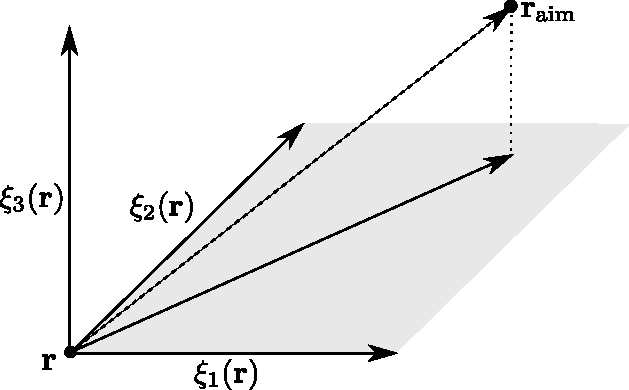
\includegraphics{fig/aim.pdf}
\caption{Illustration of algorithm for guiding trajectories in $\bm{\xi}_1(\vec{r})$ and $\bm{\xi}_2(\vec{r})$. The vector $\vec{r}_{\text{aim}}-\vec{r}$ is projected into the plane spanned by $\bm{\xi}_1(\vec{r})$ and $\bm{\xi}_2(\vec{r})$. The resulting vector is normalized and passed to the Runge-Kutta iterative solver.}\label{fig:aim}
\end{figure}

%The aim vector $\vec{\dot{r}}_{\rm{aim}}$ is continuously updated until the remaining distance separating the current position from $\vec{r}_{\rm{aim}}$ is smaller than one tenth of the initial distance $\left| \vec{r}_{\rm{aim}} - \vec{r}_0 \right|$. That is, $\vec{\dot{r}}_{\rm{aim}}$ is continuously updated as long as 

%\begin{equation}\label{eq:aim_cond}
% \left| \vec{r}_{\rm{aim}} - \vec{r}\right| > \frac{\left| \vec{r}_{\rm{aim}} - \vec{r}_0 \right|}{10}.
%\end{equation}

%As the trajectory breaks condition \eqref{eq:aim_cond}, $\vec{\dot{r}}_{\rm{aim}}$ is locked at its latest iteration. This is done in order to avoid unpredictable behavior as the trajectory approaches $\vec{r}_{\rm{aim}}$ and $\left| \vec{r}_{\rm{aim}} - \vec{r} \right|$ becomes smaller than the step length of the Runge-Kutta method.

The trajectory is terminated and the final point $\vec{r}_{\text{end}}$ returned if $\vec{r}_{\text{end}}$ satisfies equations \eqref{eq:within_dist_tol} and \eqref{eq:in_plane}. If no such point is found, the trajectory is terminated when it accumulates a length exceeding $l_{\text{max}}\left| \vec{r}_{\text{aim}} - C_i(s_k) \right|$, where $l_{\text{max}}$ is a scalar parameter greater than $1$. Here, trajectory length is computed as the sum of all constituent steps $\text{d}r$. As there is no guarantee for finding a point that satisfies both conditions \eqref{eq:within_dist_tol} and \eqref{eq:in_plane} with any given trajectory originating from $C_i$, several attempts may be needed from different initial positions.

As to limit the number of trajectories we compute in order to find any single point, we track how each trajectory is terminated. Specifically, we note whether each trajectory, corresponding to a specific start point $C_i(s_k)$ along $C_i$, reaches $\mathcal{F}_r$. If the trajectory hit $\mathcal{F}_r$, we also track whether the distance $\left|\vec{r}_{\text{end}}-M_{i,j}\right|$ overshot or undershot with regard to $\Delta_i$. For example, if we find that $\left|\vec{r}_{\text{end}}-M_{i,j}\right| < \Delta_i$, we consider the corresponding trajectory to undershoot with respect to the target point $M_{i+1,j}$. Conversely, if $\left|\vec{r}_{\text{end}}-M_{i,j}\right| > \Delta_i$, we consider the corresponding trajectory to overshoot. This feedback information allows us to dynamically choose the next initial position along $C_i$. We do this by increasing step length as long as there is no output status change, and conversely backtracking and reducing step length when a status change is detected. 

Consider the search for a new descendant point $M_{i+1,j}$ from the ancestor point $M_{i,j}$. We use an imagined trajectory originating in $M_{i,j}$ to set the initial conditions in terms of trajectory termination status. Specifically, as $M_{i,j}$ is part of $\mathcal{F}_r$, this imaginary trajectory is immediately terminated and considered as undershooting with respect to $M_{i+1,j}$. We then move by one small step $\text{d}s_{\text{min}}$ clockwise along $C_i(s)$ and compute a trajectory according to the previously outlined method. If this trajectory also reaches $\mathcal{F}_r$, undershooting with respect to $\Delta_i$, the step length $\text{d}s$ is increased by a factor $10$ before moving on. A third trajectory will then be computed using $s=s_{\text{start}}+11\text{d}s_{\text{min}}$. In general, as long as the feedback status --- that is, success at reaching $\mathcal{F}_r$ and under or overshoot with respect to $\Delta_i$ --- does not change, the step length $\text{d}s$ is increased until reaching a maximum value $\text{d}s_{\text{max}}$. However, if this feedback status changes, we backtrack to the last initial position before the status change. Then we attempt to move forward by one tenth of the last step forward. The step length is reduced by a factor of $10$ until either no status change is detected, or the minimum step length $\text{d}s_{\text{min}}$ is reached. In both of these cases we move on,  refraining from increasing the step length unless the status change was overstepped using $\text{d}s_{\text{min}}$. This process is illustrated in figure \ref{fig:d_of_s}, where we proceed from undershooting with respect to $\Delta_i$ to subsequently overshooting. Note that status changes going from overshooting to undershooting are treated in exactly the same way. This is also the case for status change regarding whether or not the trajectory reached the half-plane $\mathcal{F}_r$ before being terminated due to exceeding the maximum trajectory length $l_{\text{max}}\left|\vec{r}_{\text{aim}}-C_i(s_k)\right|$.
%terminated in or outside the half-plane $\mathcal{F}_r$.

\begin{figure}[h!] 
\centering
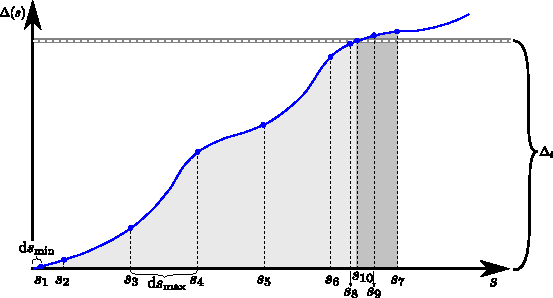
\includegraphics[width=160mm]{fig/d_of_s_2.pdf}
\caption{Illustration of algorithm for determining trajectory initial positions along the topological circle $C_i(s)$, parameterized by $s$. Along the horizontal axis is the parameter $s$ of the interpolated topological circle $C_i(s)$ on which trajectories to find new grid points are started. On the horizontal axis we correspondingly have the distance from the resulting trial point $\vec{r}_{\text{end}}$ to the ancestor point $M_{i,j}$. This distance $\left|\vec{r}_{\text{end}}-M_{i,j}\right|$ is denoted $\Delta(s)$ and assumed to be a continuous function of $s$. The target inter-levelset step length $\Delta_i$ is signified with a dashed white line within a grey field indicating the accompanying numerical tolerance (see equation \eqref{eq:within_dist_tol}). Note that $\Delta(s_{\text{start}}=0)=0$, as $M_{i,j}$ is part of the half-plane $\mathcal{F}_r$. Starting at the initial position $C_i(s_1=s_{\text{min}})$, a trajectory is developed in the ODE given by equation \eqref{eq:aim_orthogonal} until reaching the target half-plane $\mathcal{F}_r$. As the resulting distance of separation $\Delta(s_1)$, like $\Delta(s_0)$, is considered too small, $\text{d}s$ is increased by a factor of $10$ proceeding to $C_i(s_2)$. As we also have $\Delta(s_2)<\Delta_i$, $\text{d}s$ is increased once more, reaching the imposed maximum $\text{d}s_{\text{max}}$. Sucessive steps of $\text{d}s_{\text{max}}$ are then made along $C_i(s)$ until we encounter $\Delta(s_7)>\Delta_i$. Backtracking to $C_i(s_6+\text{d}s_{\text{max}}/10)$, we get $\Delta(s_8)<\Delta_i$. Reusing the same step length, we get $\Delta(s_9)>\Delta_i$, prompting the algorithm to backtrack again to $C_i(s_8+\text{d}s_{\text{max}}/100)$. This initial position $C_i(s_{10})$ yields an acceptable point, as defined by equation \eqref{eq:within_dist_tol}. Note that this dynamic step management treats any endpoint status change, including failure to reach $\mathcal{F}_r$, in the same way.}\label{fig:d_of_s}
\end{figure}

This method for choosing initial positions $C_i(s)$ along the levelset topological circle rests on the assumption that the distance $\Delta(s)=\left|\vec{r}_{\text{end}}(s)-M_{i,j}\right|$ behaves like a continuous function, possibly exhibiting asymptotic behavior near regions in which it is undefined. That is, initial positions for which the corresponding trajectories fail to reach the half-plane $\mathcal{F}_r$ within the allotted trajectory length. Based on this premise, we use the intermediate value theorem to conclude that if $\Delta(s_1) < \Delta_i$ and $\Delta(s_2) > \Delta_i$, then $\Delta(s) = \Delta_i$ for some $s$ such that $s_1<s<s_2$. In order to limit the number of necessary trajectory attempts, we therefore endeavor to move along $C_i$ with large steps wherever we are far from any intersections $\Delta(s) = \Delta_i$. However, whenever we may locate an intersection within a subdomain of $C_i(s)$, we decrease the step length $\text{d}s$ as to maximize our probability of finding this intersection. In order to manage resource requirements, we do not allow the step length to decrease beyond the minimum step length $\text{d}s_{\text{min}}$. Conversely, we limit the step from being increased beyond a maximum $\text{d}s_{\text{max}}$ as to avoid stepping over regions of two or more intersections $\Delta(s) = \Delta_i$. Note that moving past an even number of such intersections would render these intersections invisible to our method based on the intermediate value theorem, as no change in trajectory termination status would be detected.

As we anticipate asymptotic behavior close to any regions in which $\Delta(s)$ is undefined, these regions are also of great interest. We therefore manage $\text{d}s$ in the same way here as for the neighborhoods that are close to intersections $\Delta(s) = \Delta_i$. This is the case both when moving from a region in which $\Delta(s)$ is undefined and when we move into such a region. In both cases, we endeavor to find an intersection within the aforementioned possible asymptotic behavior.

In principle, all initial positions along $C_i(s)$ could be tried in order to find the new point $M_{i+1,j}$. However, trajectories from points that are far removed from $M_{i,j}$ are likely to require a long integration path, resulting in increased numerical error. Moreover, this accumulated numerical error may decrease the likelihood of reaching $\mathcal{F}_r$. In order to further limit the number of computed trajectories, we therefore restrict the choice of initial positions to points within a certain parameter interval $s_{\text{start}}\pm s_{\text{lim}}$ around the starting position. Specifically, we start by moving clockwise around $C_i(s)$ until reaching $s_{\text{start}}+s_{\text{lim}}$. We then move back to the start position $M_{i,j} = C_i(s_{\text{start}})$ and proceed counter-clockwise in the same way until reaching $s_{\text{start}}-s_{\text{lim}}$. If no new point $M_{i+1,j}$ has been found after completing this search, we prompt the exception management algorithm described in section \ref{sec:failure_management}.

%%=========================================
\subsection{Managing mesh point density and accuracy}\label{sec:grid_management}

As new levelsets $M_i$  are constructed, the distance separating neighboring points usually increases. Combined with the inter-levelset step length $\Delta_i$, these nearest-neighbor distances determine the mesh density of the computed manifold. As the point mesh $M$ is ultimately converted into a continuous manifold by use of linear interpolation (see section \ref{sec:triangulation}), we note that the accuracy of this resulting manifold depends on the mesh density of $M$. We manage this mesh density by specifying upper and lower boundaries for nearest neighbor separation, denoting these $\Delta_{\mathcal{F}}$ and $\delta_{\mathcal{F}}$, respectively. By requiring

\begin{equation}\label{eq:dist_bound_a}
\delta_{\mathcal{F}} \leq \Delta_i \leq \Delta_{\mathcal{F}}\\
\end{equation}

\noindent for the inter-levelset step length and

\begin{equation}\label{eq:dist_bound_b}
\delta_{\mathcal{F}} \leq \left| M_{i,j+1} - M_{i,j} \right| \leq \Delta_{\mathcal{F}}
\end{equation}

\noindent for levelset neighbor points, we hence limit the error of the following manifold interpolation (see section \ref{sec:triangulation}).

%interpolation error of the computed manifold according to the theory presented in section [GEODESIC LEVELSET THEORY SECTION].

After a set of descendant points $\{M_{i+1,j}\}_{j=1}^n$ have been computed from the ancestor points $\{M_{i,j}\}_{j=1}^n$, according to the previously discussed method, all nearest neighbor separation distances are reviewed. If any of these exceed $\Delta_{\mathcal{F}}$, new points are inserted inbetween. We do this by use of the same algorithm as before, except that we use ghost ancestor points, placed on $C_i$ halfway between the two nearest points. Specifically, if we have 
$\left|M_{i+1,j+1}-M_{i+1,j}\right|>\Delta_{\mathcal{F}}$, we use a ghost ancestor point $M_{i,j+1/2}$ between $M_{i,j}$ and $M_{i,j+1}$ to compute $M_{i+1,j+1/2}$. In this way, no new points are inserted using interpolations over larger separations than $\Delta_{\mathcal{F}}$. Note that as the ghost ancestor point does not itself have an ancestor to inherit a tangent vector from, $\vec{T}_{j+1/2}$ is computed as a weighted average of $\vec{T}_{j}$  and $\vec{T}_{j+1}$. This weighting is given by the distance from their respective mesh points to the ghost ancestor point.

In some cases, notably the spherical LCS described in section \ref{sec:LCS_test_cases}, nearest neighbor separation may instead decrease below $\delta_{\mathcal{F}}$. In this case, a point should be removed as long as doing so does not result in any nearest neighbor separations exceeding $\Delta_{\mathcal{F}}$. As may be seen in figure \ref{fig:grid_management}, if any of the two neighboring points may be removed without violating the upper limit of condition \eqref{eq:dist_bound_b}, the one resulting in the shortest interpoint separation is removed. If no point may be removed without violating the upper limit of condition \eqref{eq:dist_bound_b}, no action is carried out, as the minimum mesh point density threshold imposed by condition \eqref{eq:dist_bound_b} is critical in terms of limiting interpolation error.

\begin{figure}[h!] 
\centering
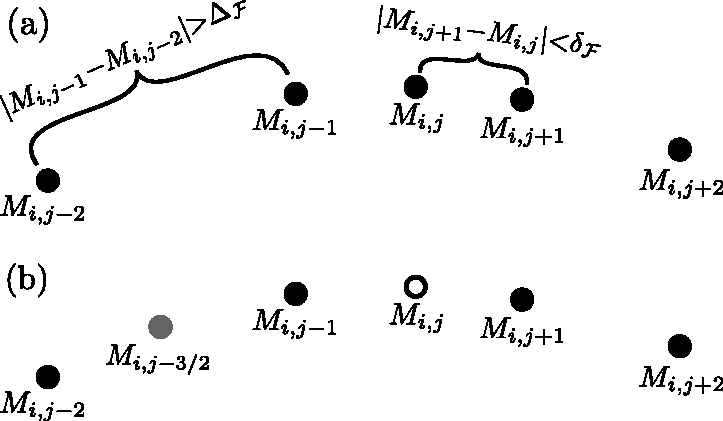
\includegraphics[width=90mm]{fig/GeodesicLevelSet_grid_management.pdf}
\caption{Mesh density management by insertion or removal of points. (a) The distance $\left|M_{i,j-1}-M_{i,j-2}\right|$ is identfied as greater than the maximum nearest neighbor distance $\Delta_{\mathcal{F}}$. Conversely, the distance $\left|M_{i,j+1}-M_{i,j}\right|$ is found to be smaller than the minimum nearest neighbor distance $\delta_{\mathcal{F}}$. (b) A new point $M_{i,j-3/2}$ is inserted between $M_{i,j-2}$ and $M_{i,j-1}$, as to keep nearest neighbor distance smaller than $\Delta_{\mathcal{F}}$. Noting that we have $\left|M_{i,j+1}-M_{i,j-1}\right|<\left|M_{i,j+2}-M_{i,j}\right|$ and $\delta_{\mathcal{F}}\leq\left|M_{i,j+1}-M_{i,j-1}\right|\leq\Delta_{\mathcal{F}}$, $M_{i,j}$ is removed to keep nearest neighbor distance larger than $\delta_{\mathcal{F}}$.}\label{fig:grid_management}
\end{figure}

%%=========================================
\subsection{Curvature-guided step management}\label{sec:step_management}

As detailed in section \ref{sec:grid_management}, all nearest neighbor manifold points are required to be separated by a distance in the range specified by conditions \eqref{eq:dist_bound_a} and \eqref{eq:dist_bound_b}. This leaves us with some flexibility with regard to choice of the inter-levelset step length $\Delta_i$. As suggested by \cite{Survey}, this is managed by monitoring local curvature. Aiming to represent local manifold behavior with appropriate detail, we adjust $\Delta_i$ dynamically. We start by defining minimum and maximum angular offset thresholds, denoting these $\alpha_{\text{min}}$ and $\alpha_{\text{max}}$, respectively. The local curvature boundary parameters $\alpha_{\text{min}}$ and $\alpha_{\text{max}}$ specify an interval of acceptable axial angle offsets $\alpha$. As illustrated in figure \ref{fig:alpha_test}, $\alpha_{i,j}$ is defined as the angular offset between the vectors $M_{i,j}-M_{i-1,j}$ and $M_{i+1,j}-M_{i,j}$, both projected into $\mathcal{F}_r$. A second analogous criterion compares the product $\alpha\Delta_i$ with corresponding upper and lower boundaries $(\Delta \alpha)_{\text{min}}$ and $(\Delta \alpha)_{\text{max}}$. By choosing appropriate bounds $(\Delta \alpha)_{\text{min}}$ and $(\Delta \alpha)_{\text{max}}$, this criterion allows us to set stricter axial angle offset requirements for large values of $\Delta_i$. Conversely, small inter-levelset step lengths $\Delta_i$ are allowed larger $\alpha$-values. In the same way, large $\Delta_i$ steps are allowed smaller $\alpha$-values. That is, we require that for each point $M_{i+1,j}$ in a new levelset we have

\begin{equation}\label{eq:curvature_test_1}
\alpha_{\text{min}} < \alpha_{i,j} < \alpha_{\text{max}}
\end{equation}

and 

\begin{equation}\label{eq:curvature_test_2}
(\Delta \alpha)_{\text{min}} < \Delta_i\alpha_{i,j} < (\Delta \alpha)_{\text{max}}.
\end{equation}

\begin{figure}[h!] 
\centering
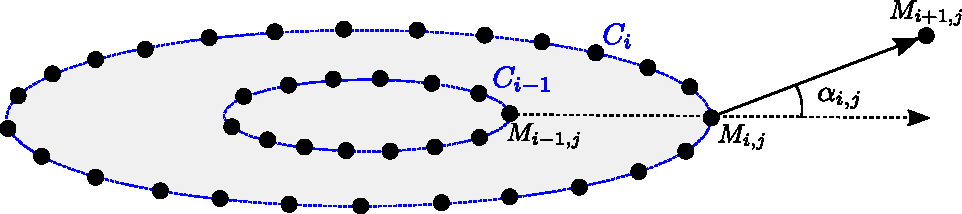
\includegraphics[width=140mm]{fig/alpha_test.pdf}
\caption{Illustration of the axial angle offset $\alpha$. We define $\alpha_{i,j}$ as the angle between the vectors $M_{i,j}-M_{i-1,j}$ and $M_{i+1,j}-M_{i,j}$.}\label{fig:alpha_test}
\end{figure}

Having completed a levelset $M_{i+1}$ of descendant points, using the step length $\Delta_i$, we review all angles $\{\alpha_{i,j}\}_{j=1}^n$. If any of these angles violate the upper thresholds (see equations \eqref{eq:curvature_test_1} and \eqref{eq:curvature_test_2}) and $\Delta_i\geq 2\delta_{\mathcal{F}}$, $M_{i+1}$ is discarded and recomputed using half the initial step-length. Conversely, if for all $\alpha_{i,j}$, both lower thresholds are violated and $2\Delta_i\leq \Delta_{\mathcal{F}}$, the levelset is kept, but the inter-levelset step length $\Delta_i$ is doubled for the next levelset. Otherwise, $\Delta_i$ is unaltered. Note that these local curvature tests are not used for inserted points. This is because an inserted point ghost ancestor does not itself have an ancestor, nor a vector $M_{i,j+1/2}-M_{i-1,j+1/2}$ from which to compute an angular offset. However, when using the inserted point $M_{i+1,j+1/2}$ as an ancestor, local curvature $\alpha_{i+1,j+1/2}$ is estimated by use of the vector $M_{i+1,j+1/2}-M_{i,j+1/2}$. That is, by use of the ghost ancestor point.

%%=========================================
\subsection{Handling failure to identify satisfactory point}\label{sec:failure_management}

As noted in section \ref{sec:trajectories}, no given trajectory from the topological circle $C_i$ is certain to produce an acceptable point in the half-plane $\mathcal{F}_r$. It is therefore possible that none of the attempted initial positions $\{C_i(s_k)\}$ along $C_i$ yield acceptable points. Since any single missing point prohibits us from computing further levelsets, proper handling of elusive points is critical.

Although impossible to guarantee, the probability of finding any given point may be significantly increased by taking appropriate measures in response to an initially failed point search. The chosen strategy was centered around introducing incremental adjustments to $\vec{r}_{\text{aim}}$, while progressively relaxing the conditions for accepting candidate points. 

Specifically, $\vec{r}_{\text{aim}}$ is adjusted by introducing an angular offset $\Delta\phi$ along the half-circle of radius $\Delta_i$ in $\mathcal{F}_r$ (see figure \ref{fig:adjust_r_aim}). Note that while the range of such angular offsets should be guided by the chosen maximal axial angle offset $\alpha_{\text{max}}$, the number of trial offsets should be guided by runtime considerations. Specifically, the angular offsets $\Delta \phi$ should roughly range from $-\alpha_{\text{max}}$ to $\alpha_{\text{max}}$, ranging most or all acceptable axial angle offsets. In this way, we attempt to correct poor initial choices of $\vec{r}_{\text{aim}}$.

\begin{figure}[h!] 
\centering
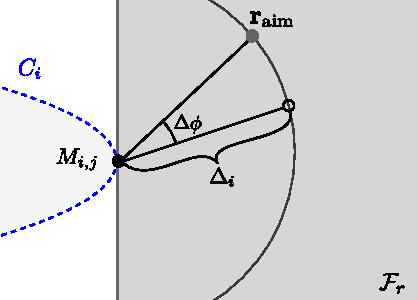
\includegraphics[width=100mm]{fig/Delta_phi.pdf}
\caption{Adjustment of $\vec{r}_{\text{aim}}$ by introducing an angular offset $\Delta\phi$ along the half-circle of radius $\Delta_i$ in $\mathcal{F}_r$. This adjustment is introduced as to account for poor initial choices of $\vec{r}_{\text{aim}}$.}\label{fig:adjust_r_aim}
\end{figure}

Having repeated the point search algorithm described in sections \ref{sec:trajectories} using all $\vec{r}_{\text{aim}}$ defined with all offsets $\{\Delta \phi\}$ without obtaining an acceptable manifold point, the conditions for point acceptance are relaxed. This is done progressively by increasing the tolerances $\Gamma_{\mathcal{F}_r}$ and $\Gamma_{\Delta}$ up to predetermined maxima $\Gamma_{\mathcal{F}_r}^{\text{max}}$ and $\Gamma_{\Delta}^{\text{max}}$. Having increased the point acceptance tolerances to their maximum values without finding an acceptable point, the incomplete levelset is discarded and recomputed with $\Delta_i = \delta_{\mathcal{F}}$. If the step length $\Delta_i$ was already set to its minimum $\delta_{\mathcal{F}}$, the procedure terminates.

%%=========================================
\subsection{Limiting accumulation of numerical noise}\label{sec:limit_numerical_noise}

Early tests of the method of geodesic levelsets indicated that error buildup over many levelsets would result in unexpected behavior for some non-analytical test fields. Specifically, small ridges in the mesh would grow for every levelset, eventually resulting in seemingly chaotic manifold structures. In some cases, this would cause loops in $C_i$, or otherwise make the manifold fold into itself. This behavior is highly problematic as manifolds described by equation \eqref{eq:hyperbolic_autonomous_dynamical_system} are by definition unable to self-intersect in any way.

In order to curb this accumulation of noise, we review each completed levelset $M_i$. Consider a point $M_{i,j}$ on this completed levelset. If any non-nearest neighbor $M_{i,j+k}$, $k > 1$ is sufficiently close to $M_{i,j}$, the intervening levelset points are removed. That is, we cut $C_i$ short whenever 
$\left| M_{i,j+k} - M_{i,j} \right|$ is sufficiently small compared to both the maximum nearest neighbor separation $\Delta_{\mathcal{F}}$ and the accumulated Euclidean nearest neighbor separations along the intervening points. Specifically, as we move along $C_i$, if for any point $M_{i,j+k}$, where $k > 1$, we have

\begin{equation}\label{eq:loop_removal_cond_a}
\left| M_{i,j+k} - M_{i,j} \right| < \Delta_{\mathcal{F}} 
\end{equation}

\noindent and

\begin{equation}\label{eq:loop_removal_cond_b}
\left| M_{i,j+k} - M_{i,j} \right| < c_{\text{arc}}\sum_{l=0}^{k-1} \left| M_{i,j+l+1} - M_{i,j+l} \right|,
\end{equation}

\noindent all points $M_{i,j+l}$ for $l=1,2,...,k-2,k-1$ are removed. Here, $c_{\text{arc}}$ is some constant $0\leq c_{\text{arc}}\leq 1$ used to control bulge tolerance. Specifically, $c_{\text{arc}}$ determines by how much arc length, represented by cumulative nearest neighbor Euclidean norm, must be reduced in order to justify point removal. That is, a large $c_{\text{arc}}$ allows for removal of blunt bulges in $C_i$, while a small $c_{\text{arc}}$ only allows for removal of sharp bulges or loops. An example demonstrating this method is displayed in figure \ref{fig:remove_loops}. Note that while possibly causing some loss of manifold detail, requiring compliance with conditions \eqref{eq:loop_removal_cond_a} and \eqref{eq:loop_removal_cond_b} prevents deletion of most conceivable large bulge formations. Also notice that since no new points are added, no error is introduced by this correction algorithm.

\begin{figure}[h!] 
\centering
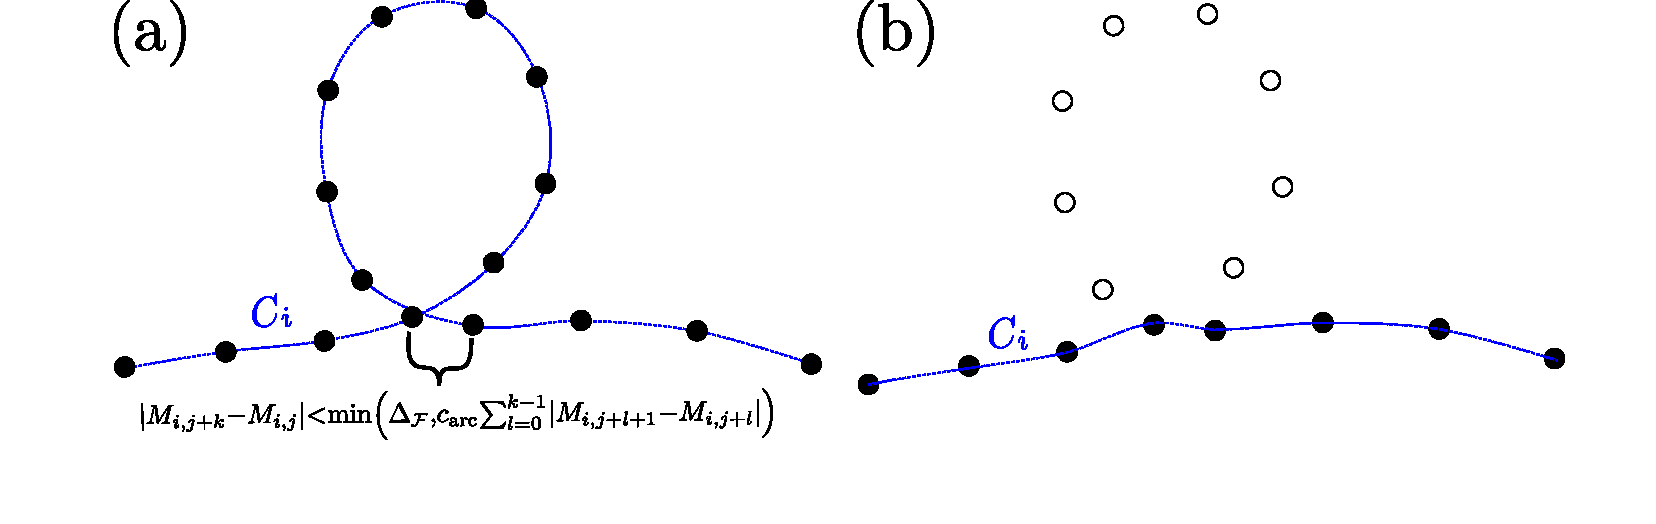
\includegraphics[width=155mm]{fig/remove_loops.pdf}
\caption{Visualization of presently described noise removal algorithm. (a) The interpoint distance $\left| M_{i,j+k} - M_{i,j}\right|$ is found to be smaller than the minimum of $\Delta_{\mathcal{F}}$ and the parameter $c_{\text{arc}}$ times the accumulated Euclidean distance between nearest neighbor points from $M_{i,j}$ to $M_{i,j+k}$. (b) The levelset points intervening between $M_{i,j}$ and $M_{i,j+k}$ have been discarded, smoothing out the corresponding topological circle $C_i$.}\label{fig:remove_loops}
\end{figure}

%Suspecting that these self-amplified ridges result from single anomalous points permanently skewing $\vec{r}_{\rm{aim}}$ for subsequent descendent points. Considering a single point associated with a large $\alpha$-offset (see section \ref{sec:step_management}), we see that the baseline axial aim angle changes for its descendent. Unless another equal and opposide axial angular offset is encountered, this point strand will continue to search for points at angles significantly different from neighboring strands. Note that while no trajectories used to find new points in $M_{i,j}$ should ever endeavor outside $\mathcal{M}$, the aim $\vec{r}_{\rm{aim}}$ how these trajectories develop inside $\mathcal{M}$. If $\vec{r}_{\rm{aim}}$ is far away from $\mathcal{M}$, some desired trajectories headed for $\mathcal{F}_r$ may not be consistent with the aim algorithm. This may lead to preferential treatment of trajectories susceptible to numerical error, likely originating from the eigenvector interpolation.

%In order to prevent formation of these self-perpetuating axial search angle errors along point strands, the vectors $\{M_{i,j}-M_{i-1,j}\}$ are reviewed for each levelset. Consider the point $M_{i,j}$ and the corresponding step vector $\vec{r}_{\rm{step},i,j} = M_{i,j}-M_{i-1,j}$. This step vector is compared to the step vector average of the two neighboring points $M_{i,j-1}$ and $M_{i,j+1}$. It is then replaced by this average if found to be sufficiently different. Specifically, the previous step vector $\vec{r}_{\rm{step},i,j}$, used to compute the subsequent aim point $\vec{r}_{\rm{aim}}$, is adjusted if

%\begin{equation}\label{eq:tol_step}
%\vec{r}_{\rm{step},i,j} \cdot \frac{\vec{r}_{\rm{step},i,j+1} + \vec{r}_{\rm{step},i,j-1}}{2} > \rm{tol}_{\rm{step}}.
%\end{equation}

%\noindent Here, $\rm{tol}_{\rm{step}}$ is a tolerance parameter directing to what extent deviation between neighboring strand search patterns is allowed. Note that while altering individual strand search focus, no points or point acceptance criteria are changed by this correction scheme.

%Another scheme analogous to the previously described step vector correction was introduced to address similar anomalies in the tangent vector $\vec{T}(\vec{r}_0)$ used to define $\mathcal{F_r}$. This is done in order to prevent point strands from converging and crossing. Again, consider a point $M_{i,j}$. Whenever the condition

%\begin{equation}\label{eq:tol_rad}
%\hat{\vec{T}}(M_{i,j}) \cdot \hat{\vec{T}}(M_{i-1,j}) > 1 - \rm{tol}_{\rm{rad}} 
%\end{equation}

%\noindent is violated, $\vec{T}(M_{i,j})$ is attempted redefined by changing the corresponding $S$-offset until condition \eqref{eq:tol_rad} is satisfied. If no iteration of $\vec{T}(M_{i,j})$ is found to satisfy condition \eqref{eq:tol_rad} the iteration most similar to the reference vector $\vec{T}(M_{i-1,j})$ is used. 



%%=========================================
\subsection{Termination criteria}\label{sec:termination_criteria}

As to avoid computing needlessly large manifolds, we define a maximum manifold size. We use geodesic distance --- the smallest distance along the manifold from $\vec{r}_0$ to the outer levelset --- as a proxy variable indicating size. This geodesic distance $r_{\mathcal{M}}$ is approximated by the sum of all completed inter-levelset steps according to 

\begin{equation}
r_{\mathcal{M}} = \sum_{i}\Delta_i.
\end{equation}

\noindent To limit manifold size, we define a maximum geodesic distance $r_{\text{max}}$, requiring the method to terminate whenever $r_{\mathcal{M}}$ exceeds $r_{\text{max}}$. This was done in order to ensure that no manifolds would become unnecessarily large, possibly straining the available memory.

A second criterion for immediate termination is implemented in order to prevent manifold self-intersections. As already noted in section \ref{sec:limit_numerical_noise}, this behavior should by definition not occur and could therefore be considered an indication of failure. Evaluating whether every new topological circle $C_i$ intersects any previous topological circle $C_{k<i}$, we define the self-intersection geodesic distance tracker variable $q$. Initially set to zero, $q$ is incremented by $\Delta_i$ whenever a new levelset $M_i$ is found to cause a self-intersection, and conversely reset to zero whenever no new self-intersections are detected. In order allow for some numerical error, we define the tolerance parameter $q_{\text{max}}$, requiring the manifold generation method to terminate whenever $q$ exceeds $q_{\text{max}}$.

Self-intersections are detected by use of triangle interpolations. As will be described in detail in section \ref{sec:triangulation}, the complete mesh $M$ is interpolated into a continuous surface by forming triangular surface elements between neighboring mesh points. This is essentially done by trilinear interpolation. Having computed a new levelset $M_i$, the area between $C_{i-1}$ and $C_i$ is covered by triangles, whereupon each new triangle is compared with all previously added triangles. If one or more of these triangles are found to intersect with any of the previously added triangles, the levelset $M_i$ is flagged as self-intersecting. Intersections between new and previously added triangles were detected with the Möller-Trumbore ray-triangle intersection algorithm, using a detection sensitivity parameter $\epsilon_{MT}=10^{-8}$ \citep{MollerTrumbore}. Our algorithm for detecting triangle intersections is outlined in figure \ref{fig:self-intersections}.

\begin{figure}[h!] 
\centering
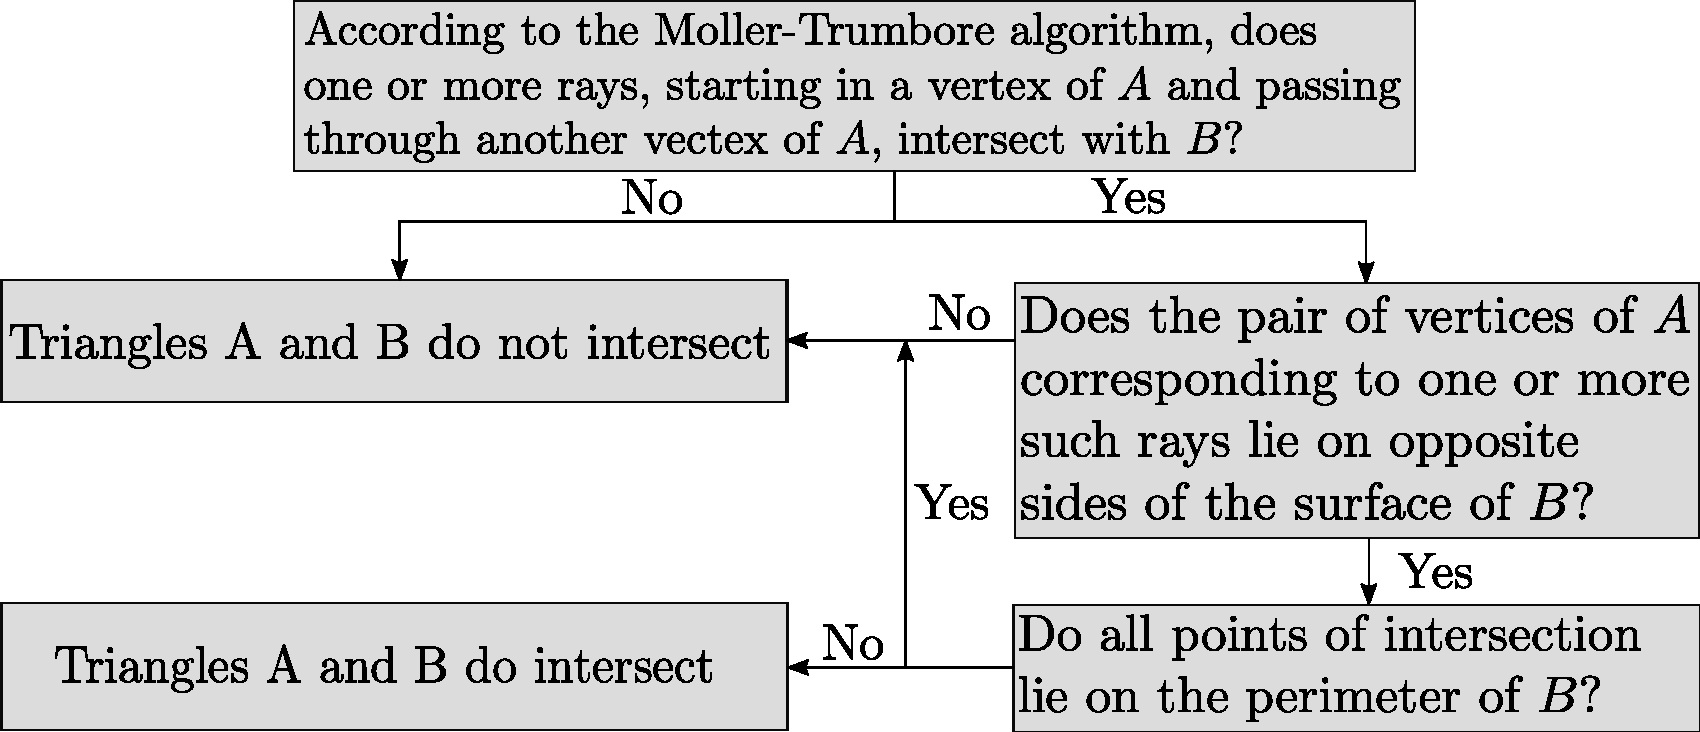
\includegraphics[width=150mm]{fig/moller_trumbore.pdf}
\caption{Flowchart describing our approach to identifying manifold self-intersections. This was done by applying the above algorithm to all interpolation triangles $A$ (see section \ref{sec:triangulation}) in a pending levelset, each compared to all previously added interpolation triangles $B$. If one or more intersections between any new triangle $A$ and and existing triangle $B$ is identified, the pending levelset is flagged as self-intersecting.}\label{fig:self-intersections}
\end{figure}

As neighboring triangles defined with the chosen triangulation approach (see section \ref{sec:triangulation}) share sides, intersections along sides were allowed. Although unlikely to occur, a side effect of allowing shared sides is that two or more triangles are also allowed to coincide perfectly. Note that this exception also allows for self-intersections, as long as the corresponding intersecting triangles do so in exactly two points, each on the sides of both triangles. This case, as well as the case of neighboring triangles, are both shown in figure \ref{fig:special_cases}. As could be expected when using the double-precision number representation, these issues were found to be insignificant. Even if a single triangle intersection is missed due to these inconsistencies, neighboring triangles are very likely to be flagged as intersecting. 
 
\begin{figure}[h!] 
\centering
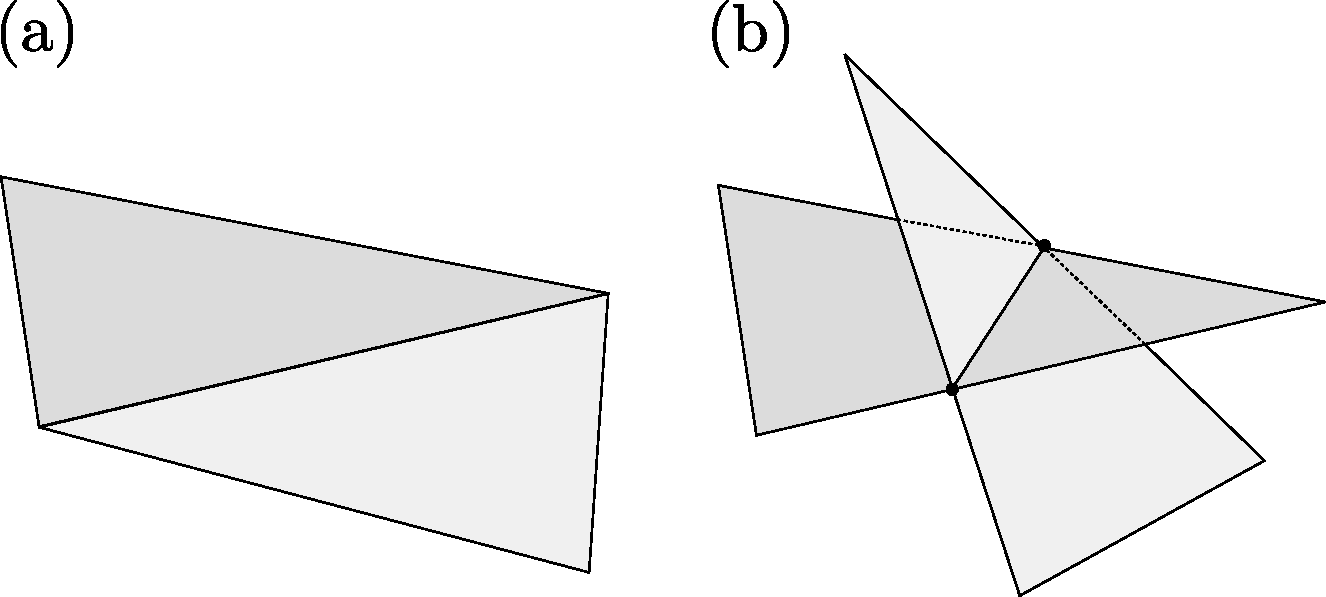
\includegraphics[width=150mm]{fig/intersections_exceptions.pdf}
\caption{Illustration of triangle intersection special cases. (a) Neighboring triangles sharing a single side are accepted as these are a natural part of our triangulation algorithm (see section \ref{sec:triangulation}). (b) Unintended, but unproblematic, case of triangle intersections evading detection from the algorithm presented in figure \ref{fig:self-intersections}. As the triangle sides intersect in exactly two points, this case is not recognized as a self-intersection.}\label{fig:special_cases}
\end{figure}

%%=========================================
\subsection{Boundary treatment}\label{sec:boundary_treatment}

The method of geodesic levelsets requires adding new points in complete levelsets forming topological circles. In addition to prohibiting addition of further points after failing to complete a single levelset, this forbids us from adding new levelsets after exceeding the domain boundaries within which the Cauchy-Green eigenvalues and eigenvectors are defined. That is, reaching these domain boundaries at a single point prohibits further development of the manifold. In order to consistently detect the manifold behavior near the boundaries of the region of interest $U$, the domain in which the Cauchy-Green eigenvalues and eigenvectors are defined should extend some distance beyond $U$. In the case of periodic systems, such as the ABC flow (see section \ref{sec:steady_abc_flow}), this is simply an exercise of utilizing this periodicity. 

In aperiodic flow fields however, this requires us to perform advection and compute eigenvalues and -vectors for an extended domain enclosing the region of interest $U$. However, in the absence of such a padding region, imposing periodic boundary conditions on the interpolated eigenvector field allows us to continue the computation --- even as parts of the manifold have left the defined domain. Note that as long as no points outside $U$ are selected as parts of the resulting LCS (see section \ref{sec:candidate_identification}), this treatment will not introduce any error unless a point strand returns to $U$ after previously having left the domain of interest. 

It should also be noted that the trajectories used to identify new mesh points are likely to reach these domain boundaries before the actual mesh points. This unpredictability may be controlled by limiting the maximal trajectory length parameter $l_{\text{max}}$ (see section \ref{sec:trajectories}).

%%=========================================
\section{Simplifying the method of geodesic levelsets by use of radial trajectories}\label{sec:force_radially_outward}

The method of geodesic levelsets was initially developed to compute manifolds defined by being everywhere tangent to a single direction field $\vec{r}'=\vec{f}(\vec{r})$. That is, an initial position in $\mathcal{M}$, transported by $\vec{f}(\vec{r})$ for any time $t$ remains within and spans the manifold $\mathcal{M}$. Assuming continuous trajectory changes while moving continuously along the topological circle $C_i$, new points are found by simply advecting these initial positions in $\vec{f}(\vec{r})$. As noted by \cite{Oettinger}, hyperbolic repelling LCSs are subsets of manifolds defined by their orthogonality to the $\bm{\xi}_3$-field. In contrast to the trajectories used by \cite{GeodesicLevelSets} and \cite{Survey}, trajectories in these manifolds are free to move within the local $\bm{\xi}_1$-$\bm{\xi}_2$-plane. That is, these trajectories have an additional degree of freedom. As described in section \ref{sec:trajectories}, this allows us to minimize trajectory travel distance by aiming each trajectory towards a position expected to be close to the next mesh point.

A more direct approach than the previously described adaptation was implemented by utilizing radial trajectories within the half-planes $\mathcal{F}_r$. These trajectories are defined by the cross product of the $\bm{\xi}_3$-field and the local tangent vector of $C$ according to

\begin{equation}\label{eq:force_radially_outward}
\vec{r}' = \bm{\xi}_3(\vec{r}) \times \vec{T}_j.
\end{equation}

\noindent The resulting direction $\vec{r}'$ is then compared with $\left|M_{i,j}-M_{i-1,j}\right|$, reversing $\vec{r}'$ if their inner product evaluates to less than zero. This approach is further illustrated in figure \ref{fig:force_radially_outward}.

\begin{figure}[h!] 
\centering
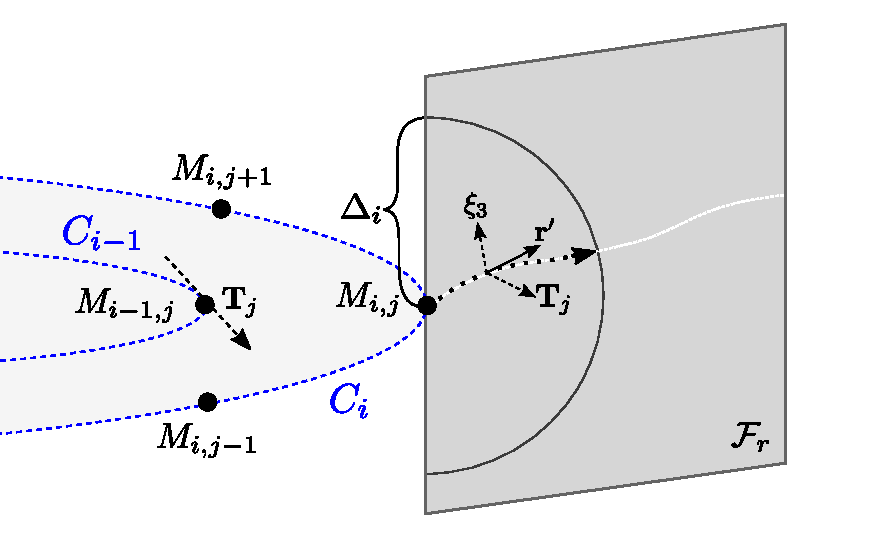
\includegraphics[width=150mm]{fig/altered_gls_trajectory.pdf}
\caption{Illustration of point search trajectories being generated by use of forced radial trajectories within the half-plane $\mathcal{F}_r$. A single trajectory is computed from the ancestor point $M_{i,j}$ by use of an adaptive step Runge-Kutta iterative ODE solver (see section \ref{sec:automatic_step_control}). The input directional vectors $\vec{r}'$ are computed as the cross product of the inherited tangent vector $\vec{T}_j$ and $\bm{\xi}_3(\vec{r})$, oriented along $M_{i,j}-M_{i-1,j}$. That is, if the inner product $\vec{r}'\cdot (M_{i,j}-M_{i-1,j})$ evaluates to less than zero, $\vec{r}'$ is reversed. The trajectory is terminated and the concluding point returned if $\left|\vec{r}-M_{i,j}\right|$ is sufficiently close to $\Delta_i$ (see equation \eqref{eq:within_dist_tol}). The white dashed line represents the intersection of the target manifold with the half-plane $\mathcal{F}_r$.}\label{fig:force_radially_outward}
\end{figure}

Using the cross product of $\bm{\xi}_3$ and the $\mathcal{F}_r$ plane normal vector $\vec{T}_j$ to compute trajectories requires special handling of the case where $\bm{\xi}_3(\vec{r}) \parallel \vec{T}_j$. This is because $\bm{\xi}_3(\vec{r}) \times \vec{T}_j$ goes to zero as $\bm{\xi}_3$ is orthogonal to $\mathcal{F}_r$. Specifically, whenever the condition

\begin{equation}\label{eq:cross_product_tolerance}
\left| \bm{\xi}_3(\vec{r}) \times \vec{T}_j\right| \geq \Gamma_{\perp}
\end{equation}

\noindent is violated, $\vec{r}'$ is copied from the last step. Here, $\Gamma_{\perp}$ is some scalar input parameter. Note that 
condition \eqref{eq:cross_product_tolerance} also serves the purpose of preventing numerical round-off error from significantly altering the computation as $\bm{\xi}_3(\vec{r}) \times \vec{T}(\vec{r})$ becomes small. Since trajectories defined by equation \eqref{eq:force_radially_outward} necessarily remain within the half-plane $\mathcal{F}_r$, equation \eqref{eq:within_dist_tol} constitutes the only remaining acceptance criterion for trajectory points. In other words, the trajectory originating from the ancestor point $M_{i,j}$ is developed according to equation \eqref{eq:force_radially_outward} until equation \eqref{eq:within_dist_tol} is satisfied. In order avoid overstepping, the Dormand-Prince method step length $\text{d}r$ is continuously limited from above according to

\begin{equation}
\text{d}r \leq \Delta_i\Gamma_{\Delta}.
\end{equation}

\noindent That is, we impose a maximum step length given by the inter-levelset step tolerance. Finally, the trajectory is terminated if no acceptable point has been found after accumulating an arc-length exceeding $l_{\text{max}}\Delta_i$, where, again, $l_{\text{max}}$ is a scalar input parameter greater than $1$. In this case, the algorithm attempts to decrease the inter-levelset step length $\Delta_i$ to $\delta_{\mathcal{F}}$ and recompute the levelset. If the failed levelset was computed using $\Delta_i=\delta_{\mathcal{F}}$, the computation is terminated.

Note that while altering trajectory development, this simplified approach of radial trajectories otherwise follows the same process as the previously described adaptation of the method of geodesic levelsets. This includes construction of the initial levelset, management of mesh density, elimination of numerical noise, and self-intersection control (see sections \ref{sec:GLS_overview}, \ref{sec:grid_management}, \ref{sec:limit_numerical_noise}, and \ref{sec:termination_criteria}, respectively). 

%%=========================================

%\subsection{Comparison of adaptation approaches for the method of geodesic levelsets}
%\label{sec:method_selection}

\section{Comparing adaptation approaches for the method of geodesic levelsets}\label{sec:method_selection}

Sections \ref{sec:GLS_intro} and \ref{sec:force_radially_outward} outline two related approaches to adapting the method of geodesic levelsets for manifolds defined by orthogonality to a vector field $\bm{\xi}_3(\vec{r})$. The first approach relies on estimating the location of new points in order to guide trajectories in $\bm{\xi}_1(\vec{r})$  and $\bm{\xi}_2(\vec{r})$. In contrast, the latter simply computes trajectories by forming the cross product of the vector $\bm{\xi}_3(\vec{r})$, to which the manifold is orthogonal, with a levelset tangent vector, inherited from the initial circular levelset $M_1$. 

While we in both approaches follow trajectories in the $\bm{\xi}_3$-orthogonal manifold and add points in a mesh of topological circles, they differ significantly both in terms of speed and consistency. The approach of forced radial trajectories within $\mathcal{F}_r$ was found to be approximately two orders of magnitude faster than the alternative method. This is because each radial trajectory is bound to the half-plane $\mathcal{F}_r$, essentially guaranteeing that it produces an acceptable mesh point as long we choose a reasonable maximum arc length $l_{\text{max}}\Delta_i$. That is, we only compute a single trajectory per new mesh point. This one-to-one relationship between computed trajectories and new mesh points is contrasted by the method of guided trajectories, where thousands of trajectories may be needed to add a single mesh point. As the probability of trajectories terminating with an acceptable mesh point is highly dependent on having an appropriate aim point, the first method also suffers heavily in terms of speed from erratic manifold behavior. Moreover, as all radial trajectory points are necessarily sufficiently close to $\mathcal{F}_r$, we only require a single acceptance criterion in the alternative approach, given by equation \eqref{eq:within_dist_tol}.

In addition to superior performance, the method of forced radial trajectories has the advantage of being significantly simpler in terms of implementation. The added complexity associated with the approach of guided trajectories is mostly due to the added task of selecting appropriate trajectory initial positions along the circle interpolation $C_i$. Moreover, the not insignificant probability of being unsuccessful in locating a specific mesh point, even after searching from initial positions along most of $C_i$, necessitates elaborate exception handling. As outlined in section \ref{sec:failure_management}, this includes adjusting the aim point while gradually relaxing our point acceptance criteria. The differences in complexity between the two considered adaptation approaches may be seen by comparing the implementation structure overviews presented in figures \ref{fig:gls_flowchart} and \ref{fig:gls_new_flowchart}.

\begin{figure}[h!] 
\centering
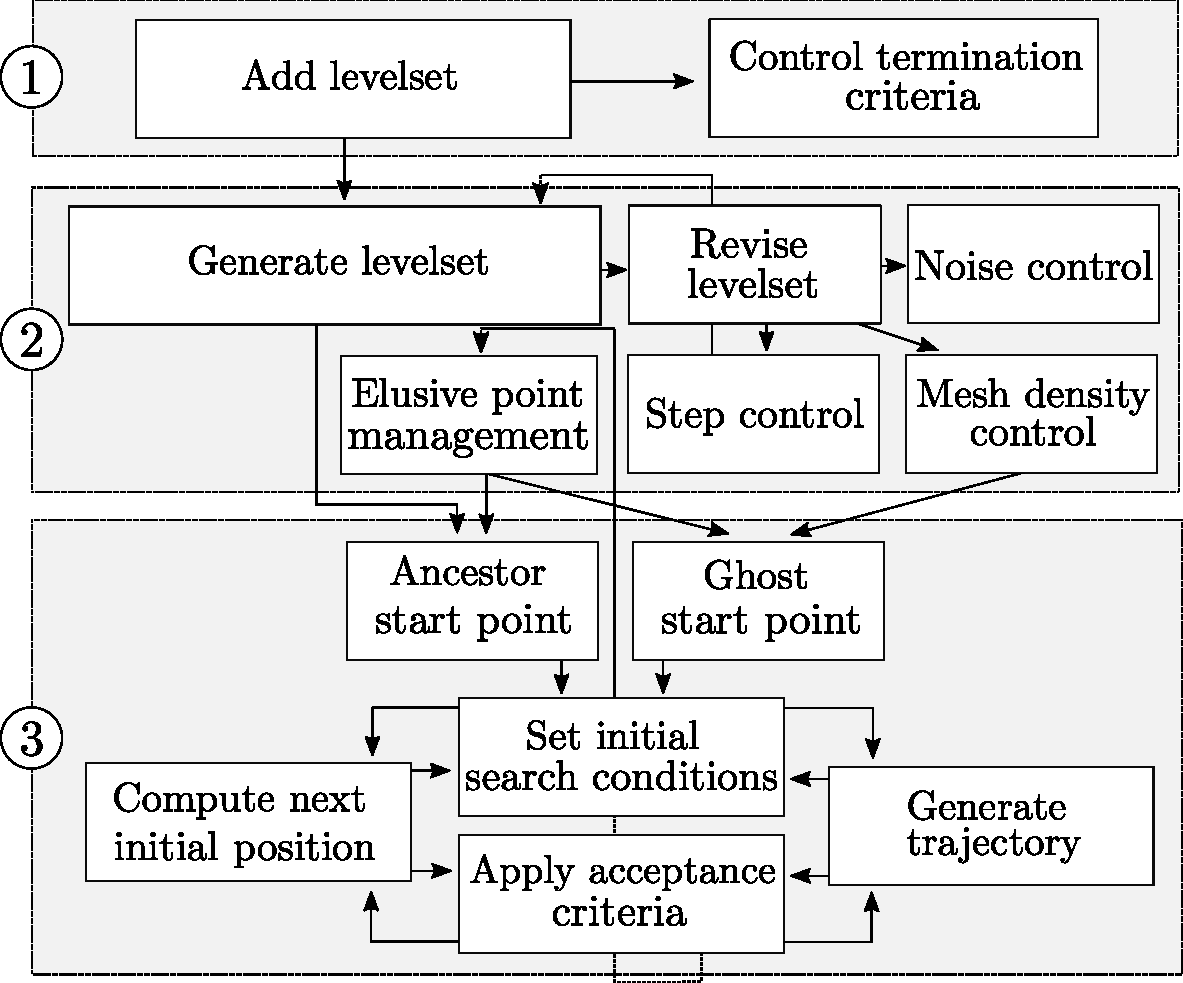
\includegraphics[width=150mm]{fig/gls_flowchart.pdf}
\caption{Outline of interaction between algorithm elements in the approach of guided trajectories. Indicating our approach to object orientation, the numbered gray fields represent our organization of the algorithm into separate layers, actualized as Python objects. (1) In the manifold layer we combine levelsets into the resulting manifold, constantly monitoring termination criteria and handling exceptions raised in the lower layer algorithm components. Specifically, this pertains to failure with regard to identifying points, prompting us to reduce inter-levelset step length $\Delta_i$, or ultimately terminate the process. (2) At the geodesic levelset layer, we combine points into sets, handling exceptions raised in the point search algorithm by calling the elusive point management algorithm (see section \ref{sec:failure_management}). This is also where suggested sets are revised by controlling mesh density, axial angle offset, and removing unnecessary bulges and loops (see sections \ref{sec:grid_management}, \ref{sec:step_management}, and \ref{sec:limit_numerical_noise}, respectively). Finally, the corresponding interpolation triangles are added (see section \ref{sec:triangulation}). (3) At the point layer, new mesh points are computed either by use of an existing ancestor point, or by a ghost ancestor point chosen from the previous topological circle $C_{i-1}$. This start point is then used to compute a trajectory in $\bm{\xi}_1(\vec{r})$ and $\bm{\xi}_2(\vec{r})$ toward the aim point $\vec{r}_{\text{aim}}$ within $\mathcal{F}_r$. This is done by first setting the initial conditions for our dynamic search for initial positions $C_i(s)$. We do this by imagining a trajectory from the start point $M_{i,j}$, immediately terminating as $M_{i,j}$ is in $\mathcal{F}_r$. Subsequent initial positions are then computed and used to generate trajectories providing feedback to the initial position selection algorithm. Whenever an acceptable point is found, it is returned to the geodesic levelset layer. Alternatively, if no such point is found an exception is raised.}\label{fig:gls_flowchart}
\end{figure}

\begin{figure}[h!] 
\centering
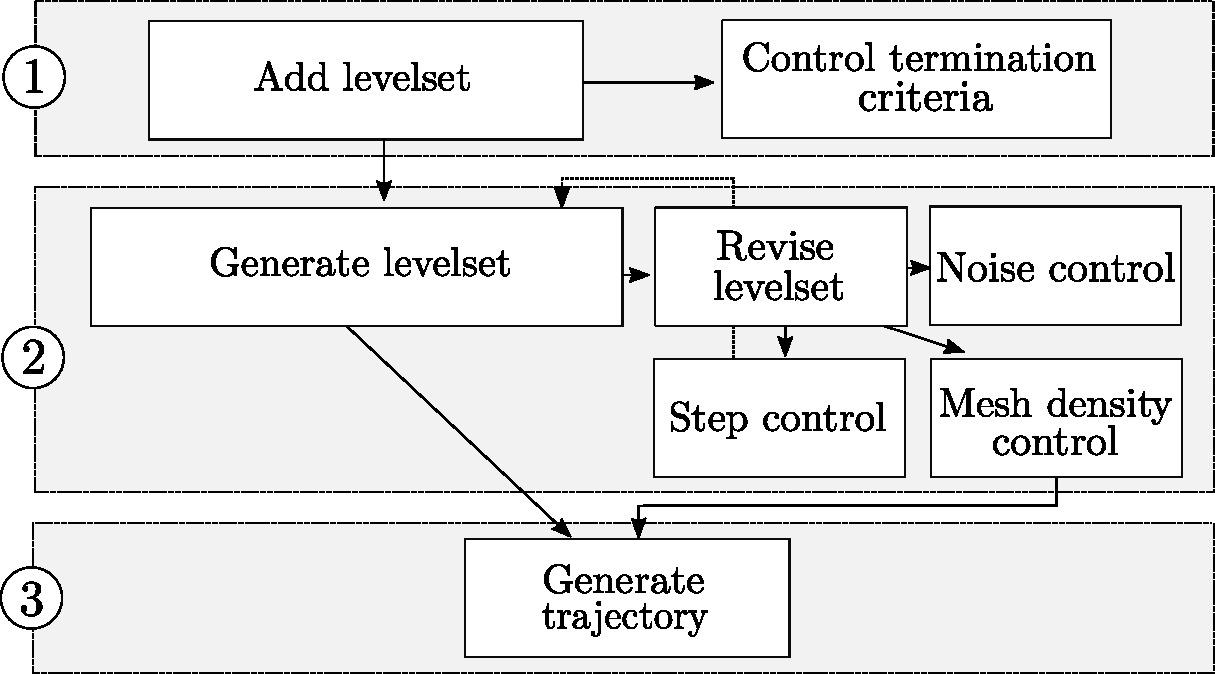
\includegraphics[width=150mm]{fig/gls_new_flowchart.pdf}
\caption{Outline of interaction between algorithm elements in the approach of radial trajectories. Indicating our approach to object orientation, the numbered gray fields represent our organization of the algorithm into separate layers, actualized as Python objects. (1) In the manifold layer we combine levelsets into the resulting manifold, constantly monitoring termination criteria and handling exceptions raised in the lower layer algorithm components. Specifically, this pertains to failure with regard to identifying points, prompting us to reduce inter-levelset step length $\Delta_i$, or ultimately terminate the process. (2) At the geodesic levelset layer we combine points into levelsets. Note that no elusive point management routine is necessary, as we are virtually guaranteed to find an acceptable point with each attempted trajectory. This is also where suggested sets are revised by controlling mesh density, axial angle offset, and removing unnecessary bulges and loops (see sections \ref{sec:grid_management}, \ref{sec:step_management}, and \ref{sec:limit_numerical_noise}, respectively). Finally, the corresponding interpolation triangles are added (see section \ref{sec:triangulation}). (3) The point layer simply consists of trajectory generation, returning acceptable points to the geodesic levelset layer. Alternatively, if no such point is found, an exception is raised. Note that failure to identify an acceptable point is very rare when using forced radial trajectories.}\label{fig:gls_new_flowchart}
\end{figure}

Like performance, the actual mesh point positions in the approach of guided trajectories were found to be sensitive to the choice of aim points. Specifically, the accuracy of this approach, in terms of reproducing reference manifolds, was found to be highly sensitive to the algorithm for selecting aim points. For example, when replacing identification of the aim point $\vec{r}_{\text{aim}}$ by linear extrapolation of $M_{i,j}-M_{i-1,j}$ with the Runge-Kutta step described in section \ref{sec:GLS_overview}, we experienced large gains both in terms of performance and accuracy. This accuracy discrepancy is surprising, as all mesh candidate points are computed by developing trajectories in $\bm{\xi}_1(\vec{r})$  and $\bm{\xi}_2(\vec{r})$, regardless of choice of aim point. Consequently, all mesh point position error should originate either from the Runge-Kutta iterative ODE solver, the initial levelset approximation (see section \ref{sec:GLS_overview}), or the topological circle interpolations $C_i$ used to insert ghost ancestor points. Although it is conceivable that these observations could be accounted for by shortening of trajectory arc lengths, hence reducing accumulated error, this behavior lessens the credibility of the approach of guided trajectories.

Due to its superior speed, consistency, and simplicity, the approach of forced radial trajectories was found preferable. All results presented in this report are generated by use of this method. It should however be noted that while deemed inferior for the purposes of this project, the approach of guided trajectories with appropriate choice of aim points, yielded practically identical results to those of forced radial trajectories in selected test cases.
 
%%=========================================
\section{Constructing manifold surfaces from point meshes}\label{sec:triangulation}

Having identified a point mesh $M$ sampled from the target manifold $\mathcal{M}$, we attempt to reproduce $\mathcal{M}$ by use of a linear interpolation scheme. Linear interpolation was chosen as implementation of higher order interpolation schemes is complicated considerably by the irregular structure of $M$.

Our primary objective for reproducing continuous manifold approximations is visual representation, rather than providing analytical expressions for $\mathcal{M}$. Therefore, no such approximated analytical expressions are computed. Instead, three-dimensional plotting algorithms, such as the triangulated surface plotting routine \texttt{plot\_}\texttt{trisurf} from the Python \textit{matplotlib} library, may be used to produce visual representations of manifolds and LCSs.

These surface plotting schemes require the use of some triangulation algorithm to define the triangular surface elements constituting a manifold. Standard triangulation algorithms such as Delaunay triangulation \citep{Delaunay} were found unsuitable for this purpose, as these do not take the specific mesh structure of $M$ into account. For instance, Delaunay triangulation was not only found to omit necessary surface triangles, but also included undesirable surface triangles, especially close to manifold creases. A custom triangulation method was therefore devised based on the method of geodesic levelsets and the corresponding mesh structure. Like in the method of geodesic levelsets, new triangles are added by starting in the manifold initial position $\vec{r}_0$ and moving progressively outwards through the levelsets $M_i$. Within a levelset $M_i$, we move clockwise around $C_i$, adding triangles covering the surface intervening between $C_i$ and $C_{i+1}$.   

As illustrated in figure \ref{fig:triangulation}, this triangulation scheme primarily  handles four main cases. In order to outline these cases, we consider a single point $M_{i,j}$. The first of these, displayed in figure \ref{fig:triangulation}\textcolor{blue}{a}, is the base case where no points have been added or removed as to manage mesh density, or eliminate numerical noise. Following the convention that triangles associated with $M_{i,j}$ should cover the surface approximating the quadrilateral $M_{i,j}M_{i,j+1}M_{i+1,j}M_{i+1,j+1}$, two triangles are added. Expressed by their vertices, these are $M_{i,j}M_{i+1,j}M_{i+1,j+1}$ and $M_{i,j}M_{i,j+1}M_{i+1,j+1}$ (see figure \ref{fig:triangulation}). Notice how, when adding quadrilaterals according to this algorithm for each point, surfaces are formed between all neighboring points within $M$. The exception to this is the surface between the manifold initial position $\vec{r}_0$ and the first topological circle $C_1$. This surface is simply reconstructed by forming triangle surfaces $\{M_0M_{1,j}M_{1,j+1}\}_{j=1}^{n}$, where $M_0$ denotes the manifold initial position $\vec{r}_0$ and $n$ is the number of points in the initial levelset. Also note the implicit convention of periodic intra-levelset numbering, that is, $M_{i,j+n}=M_{i,j}$.

\begin{figure}[h] 
\centering
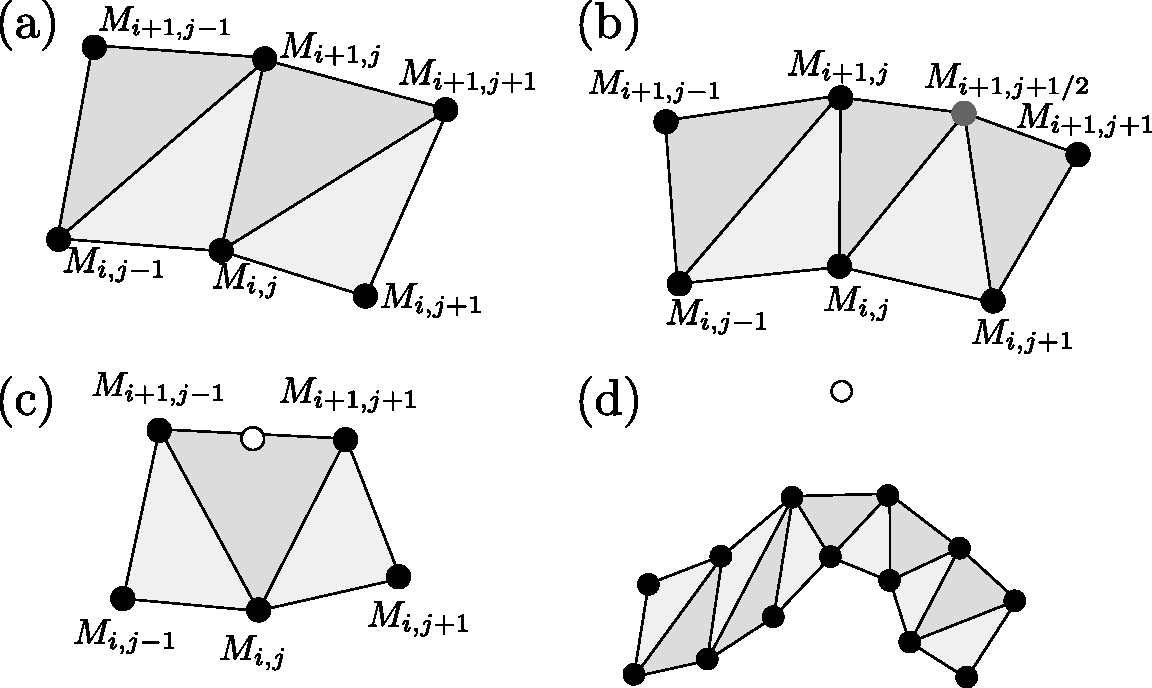
\includegraphics[width=150mm]{fig/triangulation.pdf}
\caption{Illustration of our dedicated triangulation algorithm. (a) The fundamental case where each new point has an ancestor and no points have been removed as to preserve mesh density. Associated with point $M_{i,j}$, we then insert the triangles  $M_{i,j}M_{i+1,j}M_{i+1,j+1}$ and $M_{i,j}M_{i+1,j+1}M_{i,j+1}$, each expressed by their vertices. (b) The extra point $M_{i+1,j+1/2}$ in gray has been inserted as to preserve the prescribed mesh density. Replacing the righmost quadrilateral in case (a), we now use the three triangles $M_{i,j}M_{i+1,j}M_{i+1,j+1/2}$, $M_{i,j}M_{i+1,j+1/2}M_{i,j+1}$, and $M_{i,j+1}M_{i+1,j+1/2}M_{i+1,j+1}$. (c) The point $M_{i+1,j}$ has been removed as to retain the prescribed mesh density. Here, the mesh point $M_{i,j-1}$ is merely associated with the triangle $M_{i,j-1}M_{i,j}M_{i+1,j-1}$, while $M_{i,j}$ is associated with $M_{i,j}M_{i+1,j-1}M_{i+1,j+1}$, and $M_{i,j}M_{i,j+1}M_{i+1,j+1}$. (d) A bulge has been removed. Note that while this case is handled in exactly the same way as situation (c), we could possibly be required to remove several points forming a larger bulge or loop. This instance may cause some overlap as several points in $M_{i-1}$ form triangles with the bulge-bordering points $M_{i,j}$ and $M_{i,j+k}$. However, the uncommon nature of such sudden bulges prompted us to accept this problematic case.}\label{fig:triangulation}
\end{figure} 

The two remaining cases are necessary to handle point insertion and removal. As described in sections \ref{sec:grid_management} and \ref{sec:limit_numerical_noise}, this is necessary to preserve the specified mesh density and limit accumulation of numerical noise. When an extra point $M_{i+1,j+1/2}$ is inserted between $M_{i+1,j}$ and $M_{i+1,j+1}$, the surface approximating the quadrilateral $M_{i,j}M_{i,j+1}M_{i+1,j}M_{i+1,j+1}$ is reconstructed by use of three triangular surfaces. Again expressed by their vertices, these are $M_{i,j}M_{i+1,j}M_{i+1,j+1/2}$, $M_{i,j}M_{i,j+1}M_{i+1,j+1/2}$, and $M_{i,j+1}M_{i+1,j+1/2}M_{i+1,j+1}$ (see figure \ref{fig:triangulation}\textcolor{blue}{b}).

Now, instead consider the final case where the point $M_{i+1,j}$ has been removed, either to preserve the desired mesh density, or to remove a bulge or loop. In this case, the surface approximating the two quadrilaterals $M_{i,j-1}M_{i,j}M_{i+1,j-1}M_{i+1,j}$ and $M_{i,j}M_{i,j+1}M_{i+1,j}M_{i+1,j+1}$ are reconstructed using the three triangular surfaces $M_{i,j-1}M_{i,j}M_{i+1,j-1}$, $M_{i,j}M_{i+1,j-1}M_{i+1,j+1}$, and $M_{i,j}M_{i,j+1}M_{i+1,j+1}$. This may be seen in figure \ref{fig:triangulation}\textcolor{blue}{c}. Note that the nearest neighbors of the the removed mesh point $M_{i+1,j}$ are used in these triangulations, regardless of whether these are descendant points or inserted points. As may be seen in figure \ref{fig:triangulation}\textcolor{blue}{d}, removal of loops or bulges consisting of one or more points are handled in the exact same way. Note that if several consecutive points are removed like this, the resulting triangle surface elements may be uncharacteristically large, or even partly overlap. This was however found to be a very unusual occurrence with insignificant effects on the computed LCSs.

%%=========================================
\section{Identifying repelling hyperbolic LCSs as manifold subsets}\label{sec:candidate_identification}

Starting by identifying a large number of manifolds defined by equation \eqref{eq:hyperbolic_autonomous_dynamical_system}, developed from initial positions within $U_{\text{ABD}}$, we aim to identify a sufficiently comprehensive set of surfaces that satisfy LCS condition C. That is, we identify surfaces in our domain of interest that are everywhere perpendicular to the direction of maximal repulsion. For the sake of simplicity, these initial positions are selected among the grid of tracer initial positions used to compute the flow map and its derived properties. In other words, we select the subset of these tracer initial positions that fall within $U_{\text{ABD}}$. The number of selected manifold initial positions may be controlled by superimposing a mask onto the tracer initial position grid points, evaluating only every $n_f$\ts{th} point in each direction. In this way, we effectively select initial positions within $U_{\text{ABD}}$ from a grid of prescribed density. This is done in order to reduce the number of redundant initial positions, that is, initial positions that are members of the same manifold. 

As the repelling hyperbolic LCSs of the system should be a subset of the resulting surfaces, we then proceed by applying existence criteria A, B and D to the computed manifolds. Consider a computed manifold mesh $M$. Each point $M_{i,j}$ in $M$ is reviewed and categorized based on its inclusion in $U_{\text{ABD}}$, or lack thereof. This is done by evaluating equations \eqref{eq:LCS_condition_A}, \eqref{eq:LCS_condition_B}, and \eqref{eq:LCS_condition_D}, using the interpolated eigenvalue and eigenvector fields (see section \ref{sec:Cauchy-Green_eigen}), yielding the mesh point sets $\{M_{\text{ABD}}\}$ and $\{M_{\cancel{\text{ABD}}}\}$. Note that while conditions A and B are independent of our parameter choices, D is sensitive to our choice of $\epsilon$ (see equation \eqref{eq:LCS_condition_D}). This choice determines our tolerance to offsets from the actual LCS. That is, as we compare the considered point $M_{i,j}$ with neighboring points, separated by a distance $\epsilon$ in each $\bm{\xi}_3$-direction, we could detect a peak in terms of $\lambda_3$ as long it is within the interval $[M_{i,j}-\epsilon\bm{\xi}_3(M_{i,j}),M_{i,j}+\epsilon\bm{\xi}_3(M_{i,j})]$ along $\bm{\xi}_3(M_{i,j})$. 

It seems natural to choose $\epsilon$ based on the tracer initial position grid spacing; it being indicative of the smallest scale of eigenvalue field detail. That is, if we choose $\epsilon$ larger than this grid spacing, we risk overstepping significant field behavior. Conversely, if chosen too small, we risk missing LCSs that do not pass sufficiently close by any mesh points. This is particularly crucial when selecting manifold initial positions in $U_{\text{ABD}}$ from the tracer initial position grid points, as there is no \textit{a priori} reason to assume that these points are close to the underlying LCSs. In conclusion, it seems reasonable to choose $\epsilon$ approximately one order of magnitude smaller than the tracer initial position grid spacing.

Starting from the manifold initial position --- assumed to be part of the LCS candidate --- and moving clockwise around levelsets in the order they were added, the mesh points $\{M_{\text{ABD}}\}$ are included if for any of the previously added points $\{L_k\}$

\begin{equation}
\left| M_{\text{ABD}} - L_k \right| < \Gamma_{\text{ABD}}\Delta_{\mathcal{F}}
\end{equation}

\noindent holds. That is, mesh points found to be part of $U_{\text{ABD}}$ are added if they are sufficiently close to any previously added point. This distance threshold is defined by the maximal nearest neighbor mesh point separation $\Delta_{\mathcal{F}}$ and the scalar input parameter $\Gamma_{\text{ABD}}$. In this way, we ensure that LCSs extracted from a single manifold are in fact coherent by avoiding the addition of isolated points.

Subsequently, we add all mesh points outside $U_{\text{ABD}}$, $\{M_{\cancel{\text{ABD}}}\}$, that satisfy 

\begin{equation}
\left| M_{\cancel{\text{ABD}}} - L_k \right| < \Gamma_{\text{ABD}}\Delta_{\mathcal{F}}
\end{equation}

\noindent for any $k$. Note that $\{L_k\}$ now consists of --- and is limited to --- all the previously added points from $\{M_{\text{ABD}}\}$. These new points are included in order to account for numerical error with respect to the Cauchy-Green eigenvalue and eigenvector interpolations, used to determine ABD subdomain inclusion. Moreover, they support development of continuous LCS candidate surfaces that are more conducive to analysis by inspection. Note that along with the added mesh points, we also add all the corresponding interpolation triangles for which all vertices are part of the LCS. Finally, as to smoothen out our LCS boundaries, all manifold triangle surface elements for which at least two out of three vertex points have been accepted, are added to the LCS candidate visual representation. An example of this extraction process is displayed in figure \ref{fig:LCS_extraction}.

\begin{figure}[h!]

\centering
\begin{subfigure}[b]{0.45\textwidth}
\centering
%% Creator: Matplotlib, PGF backend
%%
%% To include the figure in your LaTeX document, write
%%   \input{<filename>.pgf}
%%
%% Make sure the required packages are loaded in your preamble
%%   \usepackage{pgf}
%%
%% Figures using additional raster images can only be included by \input if
%% they are in the same directory as the main LaTeX file. For loading figures
%% from other directories you can use the `import` package
%%   \usepackage{import}
%% and then include the figures with
%%   \import{<path to file>}{<filename>.pgf}
%%
%% Matplotlib used the following preamble
%%   \usepackage{fontspec}
%%   \setmainfont{DejaVu Serif}
%%   \setsansfont{DejaVu Sans}
%%   \setmonofont{DejaVu Sans Mono}
%%
\begingroup%
\makeatletter%
\begin{pgfpicture}%
\pgfpathrectangle{\pgfpointorigin}{\pgfqpoint{2.660000in}{1.740000in}}%
\pgfusepath{use as bounding box, clip}%
\begin{pgfscope}%
\pgfsetbuttcap%
\pgfsetmiterjoin%
\definecolor{currentfill}{rgb}{1.000000,1.000000,1.000000}%
\pgfsetfillcolor{currentfill}%
\pgfsetlinewidth{0.000000pt}%
\definecolor{currentstroke}{rgb}{1.000000,1.000000,1.000000}%
\pgfsetstrokecolor{currentstroke}%
\pgfsetdash{}{0pt}%
\pgfpathmoveto{\pgfqpoint{0.000000in}{0.000000in}}%
\pgfpathlineto{\pgfqpoint{2.660000in}{0.000000in}}%
\pgfpathlineto{\pgfqpoint{2.660000in}{1.740000in}}%
\pgfpathlineto{\pgfqpoint{0.000000in}{1.740000in}}%
\pgfpathclose%
\pgfusepath{fill}%
\end{pgfscope}%
\begin{pgfscope}%
\pgfsetbuttcap%
\pgfsetmiterjoin%
\definecolor{currentfill}{rgb}{1.000000,1.000000,1.000000}%
\pgfsetfillcolor{currentfill}%
\pgfsetlinewidth{0.000000pt}%
\definecolor{currentstroke}{rgb}{0.000000,0.000000,0.000000}%
\pgfsetstrokecolor{currentstroke}%
\pgfsetstrokeopacity{0.000000}%
\pgfsetdash{}{0pt}%
\pgfpathmoveto{\pgfqpoint{-0.319200in}{0.087000in}}%
\pgfpathlineto{\pgfqpoint{2.593500in}{0.087000in}}%
\pgfpathlineto{\pgfqpoint{2.593500in}{1.774800in}}%
\pgfpathlineto{\pgfqpoint{-0.319200in}{1.774800in}}%
\pgfpathclose%
\pgfusepath{fill}%
\end{pgfscope}%
\begin{pgfscope}%
\pgfsetbuttcap%
\pgfsetmiterjoin%
\pgfsetlinewidth{0.000000pt}%
\definecolor{currentstroke}{rgb}{1.000000,1.000000,1.000000}%
\pgfsetstrokecolor{currentstroke}%
\pgfsetstrokeopacity{0.000000}%
\pgfsetdash{}{0pt}%
\pgfpathmoveto{\pgfqpoint{0.898772in}{1.254025in}}%
\pgfpathlineto{\pgfqpoint{0.094826in}{0.578837in}}%
\pgfpathlineto{\pgfqpoint{-0.008393in}{1.045696in}}%
\pgfpathlineto{\pgfqpoint{0.873475in}{1.761120in}}%
\pgfusepath{}%
\end{pgfscope}%
\begin{pgfscope}%
\pgfsetbuttcap%
\pgfsetmiterjoin%
\pgfsetlinewidth{0.000000pt}%
\definecolor{currentstroke}{rgb}{1.000000,1.000000,1.000000}%
\pgfsetstrokecolor{currentstroke}%
\pgfsetstrokeopacity{0.000000}%
\pgfsetdash{}{0pt}%
\pgfpathmoveto{\pgfqpoint{2.238643in}{0.871251in}}%
\pgfpathlineto{\pgfqpoint{0.898772in}{1.254025in}}%
\pgfpathlineto{\pgfqpoint{0.873475in}{1.761120in}}%
\pgfpathlineto{\pgfqpoint{2.337993in}{1.356234in}}%
\pgfusepath{}%
\end{pgfscope}%
\begin{pgfscope}%
\pgfsetbuttcap%
\pgfsetmiterjoin%
\pgfsetlinewidth{0.000000pt}%
\definecolor{currentstroke}{rgb}{1.000000,1.000000,1.000000}%
\pgfsetstrokecolor{currentstroke}%
\pgfsetstrokeopacity{0.000000}%
\pgfsetdash{}{0pt}%
\pgfpathmoveto{\pgfqpoint{2.238643in}{0.871251in}}%
\pgfpathlineto{\pgfqpoint{0.898772in}{1.254025in}}%
\pgfpathlineto{\pgfqpoint{0.094826in}{0.578837in}}%
\pgfpathlineto{\pgfqpoint{1.473824in}{0.161544in}}%
\pgfusepath{}%
\end{pgfscope}%
\begin{pgfscope}%
\pgfsetrectcap%
\pgfsetroundjoin%
\pgfsetlinewidth{0.803000pt}%
\definecolor{currentstroke}{rgb}{0.000000,0.000000,0.000000}%
\pgfsetstrokecolor{currentstroke}%
\pgfsetdash{}{0pt}%
\pgfpathmoveto{\pgfqpoint{0.094826in}{0.578837in}}%
\pgfpathlineto{\pgfqpoint{1.473824in}{0.161544in}}%
\pgfusepath{stroke}%
\end{pgfscope}%
\begin{pgfscope}%
\pgftext[x=0.613387in,y=0.137936in,,]{\sffamily\fontsize{10.000000}{12.000000}\selectfont \(\displaystyle x\)}%
\end{pgfscope}%
\begin{pgfscope}%
\pgfsetbuttcap%
\pgfsetroundjoin%
\pgfsetlinewidth{0.803000pt}%
\definecolor{currentstroke}{rgb}{0.690196,0.690196,0.690196}%
\pgfsetstrokecolor{currentstroke}%
\pgfsetdash{}{0pt}%
\pgfpathmoveto{\pgfqpoint{1.293646in}{0.216067in}}%
\pgfpathlineto{\pgfqpoint{2.063740in}{0.921217in}}%
\pgfpathlineto{\pgfqpoint{2.146445in}{1.409190in}}%
\pgfusepath{stroke}%
\end{pgfscope}%
\begin{pgfscope}%
\pgfsetbuttcap%
\pgfsetroundjoin%
\pgfsetlinewidth{0.803000pt}%
\definecolor{currentstroke}{rgb}{0.690196,0.690196,0.690196}%
\pgfsetstrokecolor{currentstroke}%
\pgfsetdash{}{0pt}%
\pgfpathmoveto{\pgfqpoint{0.930678in}{0.325903in}}%
\pgfpathlineto{\pgfqpoint{1.711251in}{1.021916in}}%
\pgfpathlineto{\pgfqpoint{1.760752in}{1.515820in}}%
\pgfusepath{stroke}%
\end{pgfscope}%
\begin{pgfscope}%
\pgfsetbuttcap%
\pgfsetroundjoin%
\pgfsetlinewidth{0.803000pt}%
\definecolor{currentstroke}{rgb}{0.690196,0.690196,0.690196}%
\pgfsetstrokecolor{currentstroke}%
\pgfsetdash{}{0pt}%
\pgfpathmoveto{\pgfqpoint{0.572499in}{0.434290in}}%
\pgfpathlineto{\pgfqpoint{1.363217in}{1.121342in}}%
\pgfpathlineto{\pgfqpoint{1.380381in}{1.620979in}}%
\pgfusepath{stroke}%
\end{pgfscope}%
\begin{pgfscope}%
\pgfsetbuttcap%
\pgfsetroundjoin%
\pgfsetlinewidth{0.803000pt}%
\definecolor{currentstroke}{rgb}{0.690196,0.690196,0.690196}%
\pgfsetstrokecolor{currentstroke}%
\pgfsetdash{}{0pt}%
\pgfpathmoveto{\pgfqpoint{0.219015in}{0.541257in}}%
\pgfpathlineto{\pgfqpoint{1.019554in}{1.219520in}}%
\pgfpathlineto{\pgfqpoint{1.005224in}{1.724696in}}%
\pgfusepath{stroke}%
\end{pgfscope}%
\begin{pgfscope}%
\pgfsetrectcap%
\pgfsetroundjoin%
\pgfsetlinewidth{0.803000pt}%
\definecolor{currentstroke}{rgb}{0.000000,0.000000,0.000000}%
\pgfsetstrokecolor{currentstroke}%
\pgfsetdash{}{0pt}%
\pgfpathmoveto{\pgfqpoint{1.300079in}{0.221957in}}%
\pgfpathlineto{\pgfqpoint{1.280766in}{0.204273in}}%
\pgfusepath{stroke}%
\end{pgfscope}%
\begin{pgfscope}%
\pgftext[x=1.246537in,y=0.150157in,,top]{\sffamily\fontsize{10.000000}{12.000000}\selectfont \(\displaystyle -0.5\)}%
\end{pgfscope}%
\begin{pgfscope}%
\pgfsetrectcap%
\pgfsetroundjoin%
\pgfsetlinewidth{0.803000pt}%
\definecolor{currentstroke}{rgb}{0.000000,0.000000,0.000000}%
\pgfsetstrokecolor{currentstroke}%
\pgfsetdash{}{0pt}%
\pgfpathmoveto{\pgfqpoint{0.937196in}{0.331715in}}%
\pgfpathlineto{\pgfqpoint{0.917627in}{0.314266in}}%
\pgfusepath{stroke}%
\end{pgfscope}%
\begin{pgfscope}%
\pgftext[x=0.884809in,y=0.260149in,,top]{\sffamily\fontsize{10.000000}{12.000000}\selectfont \(\displaystyle 0.0\)}%
\end{pgfscope}%
\begin{pgfscope}%
\pgfsetrectcap%
\pgfsetroundjoin%
\pgfsetlinewidth{0.803000pt}%
\definecolor{currentstroke}{rgb}{0.000000,0.000000,0.000000}%
\pgfsetstrokecolor{currentstroke}%
\pgfsetdash{}{0pt}%
\pgfpathmoveto{\pgfqpoint{0.579100in}{0.440026in}}%
\pgfpathlineto{\pgfqpoint{0.559282in}{0.422806in}}%
\pgfusepath{stroke}%
\end{pgfscope}%
\begin{pgfscope}%
\pgftext[x=0.527842in,y=0.368694in,,top]{\sffamily\fontsize{10.000000}{12.000000}\selectfont \(\displaystyle 0.5\)}%
\end{pgfscope}%
\begin{pgfscope}%
\pgfsetrectcap%
\pgfsetroundjoin%
\pgfsetlinewidth{0.803000pt}%
\definecolor{currentstroke}{rgb}{0.000000,0.000000,0.000000}%
\pgfsetstrokecolor{currentstroke}%
\pgfsetdash{}{0pt}%
\pgfpathmoveto{\pgfqpoint{0.225696in}{0.546918in}}%
\pgfpathlineto{\pgfqpoint{0.205637in}{0.529923in}}%
\pgfusepath{stroke}%
\end{pgfscope}%
\begin{pgfscope}%
\pgftext[x=0.175542in,y=0.475819in,,top]{\sffamily\fontsize{10.000000}{12.000000}\selectfont \(\displaystyle 1.0\)}%
\end{pgfscope}%
\begin{pgfscope}%
\pgfsetrectcap%
\pgfsetroundjoin%
\pgfsetlinewidth{0.803000pt}%
\definecolor{currentstroke}{rgb}{0.000000,0.000000,0.000000}%
\pgfsetstrokecolor{currentstroke}%
\pgfsetdash{}{0pt}%
\pgfpathmoveto{\pgfqpoint{2.238643in}{0.871251in}}%
\pgfpathlineto{\pgfqpoint{1.473824in}{0.161544in}}%
\pgfusepath{stroke}%
\end{pgfscope}%
\begin{pgfscope}%
\pgftext[x=2.139265in,y=0.352676in,,]{\sffamily\fontsize{10.000000}{12.000000}\selectfont \(\displaystyle y\)}%
\end{pgfscope}%
\begin{pgfscope}%
\pgfsetbuttcap%
\pgfsetroundjoin%
\pgfsetlinewidth{0.803000pt}%
\definecolor{currentstroke}{rgb}{0.690196,0.690196,0.690196}%
\pgfsetstrokecolor{currentstroke}%
\pgfsetdash{}{0pt}%
\pgfpathmoveto{\pgfqpoint{0.668795in}{1.595071in}}%
\pgfpathlineto{\pgfqpoint{0.711607in}{1.096836in}}%
\pgfpathlineto{\pgfqpoint{2.060734in}{0.706162in}}%
\pgfusepath{stroke}%
\end{pgfscope}%
\begin{pgfscope}%
\pgfsetbuttcap%
\pgfsetroundjoin%
\pgfsetlinewidth{0.803000pt}%
\definecolor{currentstroke}{rgb}{0.690196,0.690196,0.690196}%
\pgfsetstrokecolor{currentstroke}%
\pgfsetdash{}{0pt}%
\pgfpathmoveto{\pgfqpoint{0.445831in}{1.414190in}}%
\pgfpathlineto{\pgfqpoint{0.508117in}{0.925936in}}%
\pgfpathlineto{\pgfqpoint{1.867206in}{0.526579in}}%
\pgfusepath{stroke}%
\end{pgfscope}%
\begin{pgfscope}%
\pgfsetbuttcap%
\pgfsetroundjoin%
\pgfsetlinewidth{0.803000pt}%
\definecolor{currentstroke}{rgb}{0.690196,0.690196,0.690196}%
\pgfsetstrokecolor{currentstroke}%
\pgfsetdash{}{0pt}%
\pgfpathmoveto{\pgfqpoint{0.217483in}{1.228940in}}%
\pgfpathlineto{\pgfqpoint{0.300136in}{0.751264in}}%
\pgfpathlineto{\pgfqpoint{1.669298in}{0.342932in}}%
\pgfusepath{stroke}%
\end{pgfscope}%
\begin{pgfscope}%
\pgfsetrectcap%
\pgfsetroundjoin%
\pgfsetlinewidth{0.803000pt}%
\definecolor{currentstroke}{rgb}{0.000000,0.000000,0.000000}%
\pgfsetstrokecolor{currentstroke}%
\pgfsetdash{}{0pt}%
\pgfpathmoveto{\pgfqpoint{2.049674in}{0.709365in}}%
\pgfpathlineto{\pgfqpoint{2.082867in}{0.699753in}}%
\pgfusepath{stroke}%
\end{pgfscope}%
\begin{pgfscope}%
\pgftext[x=2.136188in,y=0.657976in,,top]{\sffamily\fontsize{10.000000}{12.000000}\selectfont \(\displaystyle 0.0\)}%
\end{pgfscope}%
\begin{pgfscope}%
\pgfsetrectcap%
\pgfsetroundjoin%
\pgfsetlinewidth{0.803000pt}%
\definecolor{currentstroke}{rgb}{0.000000,0.000000,0.000000}%
\pgfsetstrokecolor{currentstroke}%
\pgfsetdash{}{0pt}%
\pgfpathmoveto{\pgfqpoint{1.856061in}{0.529854in}}%
\pgfpathlineto{\pgfqpoint{1.889509in}{0.520026in}}%
\pgfusepath{stroke}%
\end{pgfscope}%
\begin{pgfscope}%
\pgftext[x=1.944196in,y=0.478501in,,top]{\sffamily\fontsize{10.000000}{12.000000}\selectfont \(\displaystyle 0.5\)}%
\end{pgfscope}%
\begin{pgfscope}%
\pgfsetrectcap%
\pgfsetroundjoin%
\pgfsetlinewidth{0.803000pt}%
\definecolor{currentstroke}{rgb}{0.000000,0.000000,0.000000}%
\pgfsetstrokecolor{currentstroke}%
\pgfsetdash{}{0pt}%
\pgfpathmoveto{\pgfqpoint{1.658067in}{0.346281in}}%
\pgfpathlineto{\pgfqpoint{1.691772in}{0.336229in}}%
\pgfusepath{stroke}%
\end{pgfscope}%
\begin{pgfscope}%
\pgftext[x=1.747875in,y=0.294978in,,top]{\sffamily\fontsize{10.000000}{12.000000}\selectfont \(\displaystyle 1.0\)}%
\end{pgfscope}%
\begin{pgfscope}%
\pgfsetrectcap%
\pgfsetroundjoin%
\pgfsetlinewidth{0.803000pt}%
\definecolor{currentstroke}{rgb}{0.000000,0.000000,0.000000}%
\pgfsetstrokecolor{currentstroke}%
\pgfsetdash{}{0pt}%
\pgfpathmoveto{\pgfqpoint{2.238643in}{0.871251in}}%
\pgfpathlineto{\pgfqpoint{2.337993in}{1.356234in}}%
\pgfusepath{stroke}%
\end{pgfscope}%
\begin{pgfscope}%
\pgftext[x=2.616448in,y=1.147329in,,]{\sffamily\fontsize{10.000000}{12.000000}\selectfont \(\displaystyle z\)}%
\end{pgfscope}%
\begin{pgfscope}%
\pgfsetbuttcap%
\pgfsetroundjoin%
\pgfsetlinewidth{0.803000pt}%
\definecolor{currentstroke}{rgb}{0.690196,0.690196,0.690196}%
\pgfsetstrokecolor{currentstroke}%
\pgfsetdash{}{0pt}%
\pgfpathmoveto{\pgfqpoint{2.248590in}{0.919812in}}%
\pgfpathlineto{\pgfqpoint{0.896234in}{1.304902in}}%
\pgfpathlineto{\pgfqpoint{0.084507in}{0.625510in}}%
\pgfusepath{stroke}%
\end{pgfscope}%
\begin{pgfscope}%
\pgfsetbuttcap%
\pgfsetroundjoin%
\pgfsetlinewidth{0.803000pt}%
\definecolor{currentstroke}{rgb}{0.690196,0.690196,0.690196}%
\pgfsetstrokecolor{currentstroke}%
\pgfsetdash{}{0pt}%
\pgfpathmoveto{\pgfqpoint{2.280545in}{1.075801in}}%
\pgfpathlineto{\pgfqpoint{0.888089in}{1.468179in}}%
\pgfpathlineto{\pgfqpoint{0.051335in}{0.775546in}}%
\pgfusepath{stroke}%
\end{pgfscope}%
\begin{pgfscope}%
\pgfsetbuttcap%
\pgfsetroundjoin%
\pgfsetlinewidth{0.803000pt}%
\definecolor{currentstroke}{rgb}{0.690196,0.690196,0.690196}%
\pgfsetstrokecolor{currentstroke}%
\pgfsetdash{}{0pt}%
\pgfpathmoveto{\pgfqpoint{2.314464in}{1.241375in}}%
\pgfpathlineto{\pgfqpoint{0.879456in}{1.641230in}}%
\pgfpathlineto{\pgfqpoint{0.016085in}{0.934984in}}%
\pgfusepath{stroke}%
\end{pgfscope}%
\begin{pgfscope}%
\pgfsetrectcap%
\pgfsetroundjoin%
\pgfsetlinewidth{0.803000pt}%
\definecolor{currentstroke}{rgb}{0.000000,0.000000,0.000000}%
\pgfsetstrokecolor{currentstroke}%
\pgfsetdash{}{0pt}%
\pgfpathmoveto{\pgfqpoint{2.237504in}{0.922968in}}%
\pgfpathlineto{\pgfqpoint{2.270776in}{0.913494in}}%
\pgfusepath{stroke}%
\end{pgfscope}%
\begin{pgfscope}%
\pgftext[x=2.371612in,y=0.936542in,,top]{\sffamily\fontsize{10.000000}{12.000000}\selectfont \(\displaystyle 1.5\)}%
\end{pgfscope}%
\begin{pgfscope}%
\pgfsetrectcap%
\pgfsetroundjoin%
\pgfsetlinewidth{0.803000pt}%
\definecolor{currentstroke}{rgb}{0.000000,0.000000,0.000000}%
\pgfsetstrokecolor{currentstroke}%
\pgfsetdash{}{0pt}%
\pgfpathmoveto{\pgfqpoint{2.269122in}{1.079020in}}%
\pgfpathlineto{\pgfqpoint{2.303406in}{1.069359in}}%
\pgfusepath{stroke}%
\end{pgfscope}%
\begin{pgfscope}%
\pgftext[x=2.407195in,y=1.092860in,,top]{\sffamily\fontsize{10.000000}{12.000000}\selectfont \(\displaystyle 2.0\)}%
\end{pgfscope}%
\begin{pgfscope}%
\pgfsetrectcap%
\pgfsetroundjoin%
\pgfsetlinewidth{0.803000pt}%
\definecolor{currentstroke}{rgb}{0.000000,0.000000,0.000000}%
\pgfsetstrokecolor{currentstroke}%
\pgfsetdash{}{0pt}%
\pgfpathmoveto{\pgfqpoint{2.302682in}{1.244658in}}%
\pgfpathlineto{\pgfqpoint{2.338041in}{1.234805in}}%
\pgfusepath{stroke}%
\end{pgfscope}%
\begin{pgfscope}%
\pgftext[x=2.444962in,y=1.258772in,,top]{\sffamily\fontsize{10.000000}{12.000000}\selectfont \(\displaystyle 2.5\)}%
\end{pgfscope}%
\begin{pgfscope}%
\pgfsys@transformshift{0.302857in}{0.452857in}%
\pgftext[left,bottom]{\pgfimage[interpolate=true,width=1.550000in,height=0.960000in]{fig/conversion-mf-small-img0.png}}%
\end{pgfscope}%
\end{pgfpicture}%
\makeatother%
\endgroup%

\caption{Sample manifold prior to LCS\\ extraction.}\label{fig:LCS_extraction_a}
\end{subfigure}
\begin{subfigure}[b]{0.45\textwidth}
\centering
%% Creator: Matplotlib, PGF backend
%%
%% To include the figure in your LaTeX document, write
%%   \input{<filename>.pgf}
%%
%% Make sure the required packages are loaded in your preamble
%%   \usepackage{pgf}
%%
%% Figures using additional raster images can only be included by \input if
%% they are in the same directory as the main LaTeX file. For loading figures
%% from other directories you can use the `import` package
%%   \usepackage{import}
%% and then include the figures with
%%   \import{<path to file>}{<filename>.pgf}
%%
%% Matplotlib used the following preamble
%%   \usepackage{fontspec}
%%   \setmainfont{DejaVu Serif}
%%   \setsansfont{DejaVu Sans}
%%   \setmonofont{DejaVu Sans Mono}
%%
\begingroup%
\makeatletter%
\begin{pgfpicture}%
\pgfpathrectangle{\pgfpointorigin}{\pgfqpoint{2.660000in}{1.740000in}}%
\pgfusepath{use as bounding box, clip}%
\begin{pgfscope}%
\pgfsetbuttcap%
\pgfsetmiterjoin%
\definecolor{currentfill}{rgb}{1.000000,1.000000,1.000000}%
\pgfsetfillcolor{currentfill}%
\pgfsetlinewidth{0.000000pt}%
\definecolor{currentstroke}{rgb}{1.000000,1.000000,1.000000}%
\pgfsetstrokecolor{currentstroke}%
\pgfsetdash{}{0pt}%
\pgfpathmoveto{\pgfqpoint{0.000000in}{0.000000in}}%
\pgfpathlineto{\pgfqpoint{2.660000in}{0.000000in}}%
\pgfpathlineto{\pgfqpoint{2.660000in}{1.740000in}}%
\pgfpathlineto{\pgfqpoint{0.000000in}{1.740000in}}%
\pgfpathclose%
\pgfusepath{fill}%
\end{pgfscope}%
\begin{pgfscope}%
\pgfsetbuttcap%
\pgfsetmiterjoin%
\definecolor{currentfill}{rgb}{1.000000,1.000000,1.000000}%
\pgfsetfillcolor{currentfill}%
\pgfsetlinewidth{0.000000pt}%
\definecolor{currentstroke}{rgb}{0.000000,0.000000,0.000000}%
\pgfsetstrokecolor{currentstroke}%
\pgfsetstrokeopacity{0.000000}%
\pgfsetdash{}{0pt}%
\pgfpathmoveto{\pgfqpoint{-0.319200in}{0.087000in}}%
\pgfpathlineto{\pgfqpoint{2.593500in}{0.087000in}}%
\pgfpathlineto{\pgfqpoint{2.593500in}{1.774800in}}%
\pgfpathlineto{\pgfqpoint{-0.319200in}{1.774800in}}%
\pgfpathclose%
\pgfusepath{fill}%
\end{pgfscope}%
\begin{pgfscope}%
\pgfsetbuttcap%
\pgfsetmiterjoin%
\pgfsetlinewidth{0.000000pt}%
\definecolor{currentstroke}{rgb}{1.000000,1.000000,1.000000}%
\pgfsetstrokecolor{currentstroke}%
\pgfsetstrokeopacity{0.000000}%
\pgfsetdash{}{0pt}%
\pgfpathmoveto{\pgfqpoint{0.898772in}{1.254025in}}%
\pgfpathlineto{\pgfqpoint{0.094826in}{0.578837in}}%
\pgfpathlineto{\pgfqpoint{-0.008393in}{1.045696in}}%
\pgfpathlineto{\pgfqpoint{0.873475in}{1.761120in}}%
\pgfusepath{}%
\end{pgfscope}%
\begin{pgfscope}%
\pgfsetbuttcap%
\pgfsetmiterjoin%
\pgfsetlinewidth{0.000000pt}%
\definecolor{currentstroke}{rgb}{1.000000,1.000000,1.000000}%
\pgfsetstrokecolor{currentstroke}%
\pgfsetstrokeopacity{0.000000}%
\pgfsetdash{}{0pt}%
\pgfpathmoveto{\pgfqpoint{2.238643in}{0.871251in}}%
\pgfpathlineto{\pgfqpoint{0.898772in}{1.254025in}}%
\pgfpathlineto{\pgfqpoint{0.873475in}{1.761120in}}%
\pgfpathlineto{\pgfqpoint{2.337993in}{1.356234in}}%
\pgfusepath{}%
\end{pgfscope}%
\begin{pgfscope}%
\pgfsetbuttcap%
\pgfsetmiterjoin%
\pgfsetlinewidth{0.000000pt}%
\definecolor{currentstroke}{rgb}{1.000000,1.000000,1.000000}%
\pgfsetstrokecolor{currentstroke}%
\pgfsetstrokeopacity{0.000000}%
\pgfsetdash{}{0pt}%
\pgfpathmoveto{\pgfqpoint{2.238643in}{0.871251in}}%
\pgfpathlineto{\pgfqpoint{0.898772in}{1.254025in}}%
\pgfpathlineto{\pgfqpoint{0.094826in}{0.578837in}}%
\pgfpathlineto{\pgfqpoint{1.473824in}{0.161544in}}%
\pgfusepath{}%
\end{pgfscope}%
\begin{pgfscope}%
\pgfsetrectcap%
\pgfsetroundjoin%
\pgfsetlinewidth{0.803000pt}%
\definecolor{currentstroke}{rgb}{0.000000,0.000000,0.000000}%
\pgfsetstrokecolor{currentstroke}%
\pgfsetdash{}{0pt}%
\pgfpathmoveto{\pgfqpoint{0.094826in}{0.578837in}}%
\pgfpathlineto{\pgfqpoint{1.473824in}{0.161544in}}%
\pgfusepath{stroke}%
\end{pgfscope}%
\begin{pgfscope}%
\pgftext[x=0.613387in,y=0.137936in,,]{\sffamily\fontsize{10.000000}{12.000000}\selectfont \(\displaystyle x\)}%
\end{pgfscope}%
\begin{pgfscope}%
\pgfsetbuttcap%
\pgfsetroundjoin%
\pgfsetlinewidth{0.803000pt}%
\definecolor{currentstroke}{rgb}{0.690196,0.690196,0.690196}%
\pgfsetstrokecolor{currentstroke}%
\pgfsetdash{}{0pt}%
\pgfpathmoveto{\pgfqpoint{1.293646in}{0.216067in}}%
\pgfpathlineto{\pgfqpoint{2.063740in}{0.921217in}}%
\pgfpathlineto{\pgfqpoint{2.146445in}{1.409190in}}%
\pgfusepath{stroke}%
\end{pgfscope}%
\begin{pgfscope}%
\pgfsetbuttcap%
\pgfsetroundjoin%
\pgfsetlinewidth{0.803000pt}%
\definecolor{currentstroke}{rgb}{0.690196,0.690196,0.690196}%
\pgfsetstrokecolor{currentstroke}%
\pgfsetdash{}{0pt}%
\pgfpathmoveto{\pgfqpoint{0.930678in}{0.325903in}}%
\pgfpathlineto{\pgfqpoint{1.711251in}{1.021916in}}%
\pgfpathlineto{\pgfqpoint{1.760752in}{1.515820in}}%
\pgfusepath{stroke}%
\end{pgfscope}%
\begin{pgfscope}%
\pgfsetbuttcap%
\pgfsetroundjoin%
\pgfsetlinewidth{0.803000pt}%
\definecolor{currentstroke}{rgb}{0.690196,0.690196,0.690196}%
\pgfsetstrokecolor{currentstroke}%
\pgfsetdash{}{0pt}%
\pgfpathmoveto{\pgfqpoint{0.572499in}{0.434290in}}%
\pgfpathlineto{\pgfqpoint{1.363217in}{1.121342in}}%
\pgfpathlineto{\pgfqpoint{1.380381in}{1.620979in}}%
\pgfusepath{stroke}%
\end{pgfscope}%
\begin{pgfscope}%
\pgfsetbuttcap%
\pgfsetroundjoin%
\pgfsetlinewidth{0.803000pt}%
\definecolor{currentstroke}{rgb}{0.690196,0.690196,0.690196}%
\pgfsetstrokecolor{currentstroke}%
\pgfsetdash{}{0pt}%
\pgfpathmoveto{\pgfqpoint{0.219015in}{0.541257in}}%
\pgfpathlineto{\pgfqpoint{1.019554in}{1.219520in}}%
\pgfpathlineto{\pgfqpoint{1.005224in}{1.724696in}}%
\pgfusepath{stroke}%
\end{pgfscope}%
\begin{pgfscope}%
\pgfsetrectcap%
\pgfsetroundjoin%
\pgfsetlinewidth{0.803000pt}%
\definecolor{currentstroke}{rgb}{0.000000,0.000000,0.000000}%
\pgfsetstrokecolor{currentstroke}%
\pgfsetdash{}{0pt}%
\pgfpathmoveto{\pgfqpoint{1.300079in}{0.221957in}}%
\pgfpathlineto{\pgfqpoint{1.280766in}{0.204273in}}%
\pgfusepath{stroke}%
\end{pgfscope}%
\begin{pgfscope}%
\pgftext[x=1.246537in,y=0.150157in,,top]{\sffamily\fontsize{10.000000}{12.000000}\selectfont \(\displaystyle -0.5\)}%
\end{pgfscope}%
\begin{pgfscope}%
\pgfsetrectcap%
\pgfsetroundjoin%
\pgfsetlinewidth{0.803000pt}%
\definecolor{currentstroke}{rgb}{0.000000,0.000000,0.000000}%
\pgfsetstrokecolor{currentstroke}%
\pgfsetdash{}{0pt}%
\pgfpathmoveto{\pgfqpoint{0.937196in}{0.331715in}}%
\pgfpathlineto{\pgfqpoint{0.917627in}{0.314266in}}%
\pgfusepath{stroke}%
\end{pgfscope}%
\begin{pgfscope}%
\pgftext[x=0.884809in,y=0.260149in,,top]{\sffamily\fontsize{10.000000}{12.000000}\selectfont \(\displaystyle 0.0\)}%
\end{pgfscope}%
\begin{pgfscope}%
\pgfsetrectcap%
\pgfsetroundjoin%
\pgfsetlinewidth{0.803000pt}%
\definecolor{currentstroke}{rgb}{0.000000,0.000000,0.000000}%
\pgfsetstrokecolor{currentstroke}%
\pgfsetdash{}{0pt}%
\pgfpathmoveto{\pgfqpoint{0.579100in}{0.440026in}}%
\pgfpathlineto{\pgfqpoint{0.559282in}{0.422806in}}%
\pgfusepath{stroke}%
\end{pgfscope}%
\begin{pgfscope}%
\pgftext[x=0.527842in,y=0.368694in,,top]{\sffamily\fontsize{10.000000}{12.000000}\selectfont \(\displaystyle 0.5\)}%
\end{pgfscope}%
\begin{pgfscope}%
\pgfsetrectcap%
\pgfsetroundjoin%
\pgfsetlinewidth{0.803000pt}%
\definecolor{currentstroke}{rgb}{0.000000,0.000000,0.000000}%
\pgfsetstrokecolor{currentstroke}%
\pgfsetdash{}{0pt}%
\pgfpathmoveto{\pgfqpoint{0.225696in}{0.546918in}}%
\pgfpathlineto{\pgfqpoint{0.205637in}{0.529923in}}%
\pgfusepath{stroke}%
\end{pgfscope}%
\begin{pgfscope}%
\pgftext[x=0.175542in,y=0.475819in,,top]{\sffamily\fontsize{10.000000}{12.000000}\selectfont \(\displaystyle 1.0\)}%
\end{pgfscope}%
\begin{pgfscope}%
\pgfsetrectcap%
\pgfsetroundjoin%
\pgfsetlinewidth{0.803000pt}%
\definecolor{currentstroke}{rgb}{0.000000,0.000000,0.000000}%
\pgfsetstrokecolor{currentstroke}%
\pgfsetdash{}{0pt}%
\pgfpathmoveto{\pgfqpoint{2.238643in}{0.871251in}}%
\pgfpathlineto{\pgfqpoint{1.473824in}{0.161544in}}%
\pgfusepath{stroke}%
\end{pgfscope}%
\begin{pgfscope}%
\pgftext[x=2.139265in,y=0.352676in,,]{\sffamily\fontsize{10.000000}{12.000000}\selectfont \(\displaystyle y\)}%
\end{pgfscope}%
\begin{pgfscope}%
\pgfsetbuttcap%
\pgfsetroundjoin%
\pgfsetlinewidth{0.803000pt}%
\definecolor{currentstroke}{rgb}{0.690196,0.690196,0.690196}%
\pgfsetstrokecolor{currentstroke}%
\pgfsetdash{}{0pt}%
\pgfpathmoveto{\pgfqpoint{0.668795in}{1.595071in}}%
\pgfpathlineto{\pgfqpoint{0.711607in}{1.096836in}}%
\pgfpathlineto{\pgfqpoint{2.060734in}{0.706162in}}%
\pgfusepath{stroke}%
\end{pgfscope}%
\begin{pgfscope}%
\pgfsetbuttcap%
\pgfsetroundjoin%
\pgfsetlinewidth{0.803000pt}%
\definecolor{currentstroke}{rgb}{0.690196,0.690196,0.690196}%
\pgfsetstrokecolor{currentstroke}%
\pgfsetdash{}{0pt}%
\pgfpathmoveto{\pgfqpoint{0.445831in}{1.414190in}}%
\pgfpathlineto{\pgfqpoint{0.508117in}{0.925936in}}%
\pgfpathlineto{\pgfqpoint{1.867206in}{0.526579in}}%
\pgfusepath{stroke}%
\end{pgfscope}%
\begin{pgfscope}%
\pgfsetbuttcap%
\pgfsetroundjoin%
\pgfsetlinewidth{0.803000pt}%
\definecolor{currentstroke}{rgb}{0.690196,0.690196,0.690196}%
\pgfsetstrokecolor{currentstroke}%
\pgfsetdash{}{0pt}%
\pgfpathmoveto{\pgfqpoint{0.217483in}{1.228940in}}%
\pgfpathlineto{\pgfqpoint{0.300136in}{0.751264in}}%
\pgfpathlineto{\pgfqpoint{1.669298in}{0.342932in}}%
\pgfusepath{stroke}%
\end{pgfscope}%
\begin{pgfscope}%
\pgfsetrectcap%
\pgfsetroundjoin%
\pgfsetlinewidth{0.803000pt}%
\definecolor{currentstroke}{rgb}{0.000000,0.000000,0.000000}%
\pgfsetstrokecolor{currentstroke}%
\pgfsetdash{}{0pt}%
\pgfpathmoveto{\pgfqpoint{2.049674in}{0.709365in}}%
\pgfpathlineto{\pgfqpoint{2.082867in}{0.699753in}}%
\pgfusepath{stroke}%
\end{pgfscope}%
\begin{pgfscope}%
\pgftext[x=2.136188in,y=0.657976in,,top]{\sffamily\fontsize{10.000000}{12.000000}\selectfont \(\displaystyle 0.0\)}%
\end{pgfscope}%
\begin{pgfscope}%
\pgfsetrectcap%
\pgfsetroundjoin%
\pgfsetlinewidth{0.803000pt}%
\definecolor{currentstroke}{rgb}{0.000000,0.000000,0.000000}%
\pgfsetstrokecolor{currentstroke}%
\pgfsetdash{}{0pt}%
\pgfpathmoveto{\pgfqpoint{1.856061in}{0.529854in}}%
\pgfpathlineto{\pgfqpoint{1.889509in}{0.520026in}}%
\pgfusepath{stroke}%
\end{pgfscope}%
\begin{pgfscope}%
\pgftext[x=1.944196in,y=0.478501in,,top]{\sffamily\fontsize{10.000000}{12.000000}\selectfont \(\displaystyle 0.5\)}%
\end{pgfscope}%
\begin{pgfscope}%
\pgfsetrectcap%
\pgfsetroundjoin%
\pgfsetlinewidth{0.803000pt}%
\definecolor{currentstroke}{rgb}{0.000000,0.000000,0.000000}%
\pgfsetstrokecolor{currentstroke}%
\pgfsetdash{}{0pt}%
\pgfpathmoveto{\pgfqpoint{1.658067in}{0.346281in}}%
\pgfpathlineto{\pgfqpoint{1.691772in}{0.336229in}}%
\pgfusepath{stroke}%
\end{pgfscope}%
\begin{pgfscope}%
\pgftext[x=1.747875in,y=0.294978in,,top]{\sffamily\fontsize{10.000000}{12.000000}\selectfont \(\displaystyle 1.0\)}%
\end{pgfscope}%
\begin{pgfscope}%
\pgfsetrectcap%
\pgfsetroundjoin%
\pgfsetlinewidth{0.803000pt}%
\definecolor{currentstroke}{rgb}{0.000000,0.000000,0.000000}%
\pgfsetstrokecolor{currentstroke}%
\pgfsetdash{}{0pt}%
\pgfpathmoveto{\pgfqpoint{2.238643in}{0.871251in}}%
\pgfpathlineto{\pgfqpoint{2.337993in}{1.356234in}}%
\pgfusepath{stroke}%
\end{pgfscope}%
\begin{pgfscope}%
\pgftext[x=2.616448in,y=1.147329in,,]{\sffamily\fontsize{10.000000}{12.000000}\selectfont \(\displaystyle z\)}%
\end{pgfscope}%
\begin{pgfscope}%
\pgfsetbuttcap%
\pgfsetroundjoin%
\pgfsetlinewidth{0.803000pt}%
\definecolor{currentstroke}{rgb}{0.690196,0.690196,0.690196}%
\pgfsetstrokecolor{currentstroke}%
\pgfsetdash{}{0pt}%
\pgfpathmoveto{\pgfqpoint{2.248590in}{0.919812in}}%
\pgfpathlineto{\pgfqpoint{0.896234in}{1.304902in}}%
\pgfpathlineto{\pgfqpoint{0.084507in}{0.625510in}}%
\pgfusepath{stroke}%
\end{pgfscope}%
\begin{pgfscope}%
\pgfsetbuttcap%
\pgfsetroundjoin%
\pgfsetlinewidth{0.803000pt}%
\definecolor{currentstroke}{rgb}{0.690196,0.690196,0.690196}%
\pgfsetstrokecolor{currentstroke}%
\pgfsetdash{}{0pt}%
\pgfpathmoveto{\pgfqpoint{2.280545in}{1.075801in}}%
\pgfpathlineto{\pgfqpoint{0.888089in}{1.468179in}}%
\pgfpathlineto{\pgfqpoint{0.051335in}{0.775546in}}%
\pgfusepath{stroke}%
\end{pgfscope}%
\begin{pgfscope}%
\pgfsetbuttcap%
\pgfsetroundjoin%
\pgfsetlinewidth{0.803000pt}%
\definecolor{currentstroke}{rgb}{0.690196,0.690196,0.690196}%
\pgfsetstrokecolor{currentstroke}%
\pgfsetdash{}{0pt}%
\pgfpathmoveto{\pgfqpoint{2.314464in}{1.241375in}}%
\pgfpathlineto{\pgfqpoint{0.879456in}{1.641230in}}%
\pgfpathlineto{\pgfqpoint{0.016085in}{0.934984in}}%
\pgfusepath{stroke}%
\end{pgfscope}%
\begin{pgfscope}%
\pgfsetrectcap%
\pgfsetroundjoin%
\pgfsetlinewidth{0.803000pt}%
\definecolor{currentstroke}{rgb}{0.000000,0.000000,0.000000}%
\pgfsetstrokecolor{currentstroke}%
\pgfsetdash{}{0pt}%
\pgfpathmoveto{\pgfqpoint{2.237504in}{0.922968in}}%
\pgfpathlineto{\pgfqpoint{2.270776in}{0.913494in}}%
\pgfusepath{stroke}%
\end{pgfscope}%
\begin{pgfscope}%
\pgftext[x=2.371612in,y=0.936542in,,top]{\sffamily\fontsize{10.000000}{12.000000}\selectfont \(\displaystyle 1.5\)}%
\end{pgfscope}%
\begin{pgfscope}%
\pgfsetrectcap%
\pgfsetroundjoin%
\pgfsetlinewidth{0.803000pt}%
\definecolor{currentstroke}{rgb}{0.000000,0.000000,0.000000}%
\pgfsetstrokecolor{currentstroke}%
\pgfsetdash{}{0pt}%
\pgfpathmoveto{\pgfqpoint{2.269122in}{1.079020in}}%
\pgfpathlineto{\pgfqpoint{2.303406in}{1.069359in}}%
\pgfusepath{stroke}%
\end{pgfscope}%
\begin{pgfscope}%
\pgftext[x=2.407195in,y=1.092860in,,top]{\sffamily\fontsize{10.000000}{12.000000}\selectfont \(\displaystyle 2.0\)}%
\end{pgfscope}%
\begin{pgfscope}%
\pgfsetrectcap%
\pgfsetroundjoin%
\pgfsetlinewidth{0.803000pt}%
\definecolor{currentstroke}{rgb}{0.000000,0.000000,0.000000}%
\pgfsetstrokecolor{currentstroke}%
\pgfsetdash{}{0pt}%
\pgfpathmoveto{\pgfqpoint{2.302682in}{1.244658in}}%
\pgfpathlineto{\pgfqpoint{2.338041in}{1.234805in}}%
\pgfusepath{stroke}%
\end{pgfscope}%
\begin{pgfscope}%
\pgftext[x=2.444962in,y=1.258772in,,top]{\sffamily\fontsize{10.000000}{12.000000}\selectfont \(\displaystyle 2.5\)}%
\end{pgfscope}%
\begin{pgfscope}%
\pgfsys@transformshift{0.302857in}{0.465714in}%
\pgftext[left,bottom]{\pgfimage[interpolate=true,width=1.098571in,height=0.885714in]{fig/conversion-lcs-small-img0.png}}%
\end{pgfscope}%
\end{pgfpicture}%
\makeatother%
\endgroup%

\caption{Extracted LCS from sample manifold displayed in (a).}\label{fig:LCS_extraction_b}
\end{subfigure}

\caption{LCS extraction from sample manifold. The sample manifold was computed using the steady ABC flow system described in section \ref{sec:steady_abc_flow}.}\label{fig:LCS_extraction} 
\end{figure}

Having extracted the manifold subsets on which conditions A, B, and D (see equations \eqref{eq:LCS_condition_A}, \eqref{eq:LCS_condition_B}, and \eqref{eq:LCS_condition_D}) are satisfied, we are left with surfaces that, when allowing for some numerical error, have been determined to comply with all the LCS acceptance criteria proposed by \cite{Haller14Errata}. In the interest of clarity, the smallest LCS candidates are discarded, as these may be expected to have limited impact on the flow system \citep{Haller12}. This is done by computing LCS area according to equation \ref{eq:compute_area} and defining a minimum area threshold $A_{\text{min}}$. Finally, as a sanity check, any LCS candidates with average repulsion $\bar{\lambda}_3$ smaller than 1, are removed. This is done to ensure that all identified repelling hyperbolic LCS are in fact repelling, as established by condition A. The remaining LCS candidates are then accepted as repelling hyperbolic LCSs.

The repulsion average $\overline{\lambda}_3$ was determined for each LCS candidate surface by a weighted average of $\lambda_3$, evaluated at all its constituent points. Note that, as the interpolated eigenvalue field may exhibit oscillatory behavior, some points were found to exhibit $\lambda_3$-values several orders of magnitude different from all neighboring points. In order to prevent small numbers of outlier points from severely skewing $\overline{\lambda}_3$, some data points were neglected. Specifically, the adjusted repulsion average $\widehat{\lambda}_3$ was computed iteratively by alternately removing $\text{max}(\lambda_3)$ and $\text{min}(\lambda_3)$. Each adjustment was then accepted if

\begin{equation}\label{eq:adjust_lambda_3}
\left| \frac{\overline{\lambda}_3}{\widehat{\lambda}_3} - 1\right| > 0.1,
\end{equation}

\noindent prompting us to accept $\widehat{\lambda}_3$ as the new baseline average $\overline{\lambda}_3$. These adjustments were repeated until neither $\text{max}(\lambda_3)$ nor $\text{min}(\lambda_3)$ could be removed without violating condition \eqref{eq:adjust_lambda_3}. 

The weighting of this repulsion average was chosen to approximate the surface area represented by each sampled point $M_{i,j}$. Specifically, the weight of $M_{i,j}$, $W_{i,j}$, was computed as 

\begin{equation}
W_{i,j} = \frac{\Delta_{i}+\Delta_{i-1}}{2}\frac{\left|M_{i,j}-M_{i,j-1}\right|+\left|M_{i,j+1}-M_{i,j}\right|}{2}.
\end{equation}

\noindent That is, the weight of each manifold point $M_{i,j}$ is defined as to approximate the region of $\mathcal{M}$ that is closer to $M_{i,j}$ than to any other mesh point in $M$. The physical analogue to this weighting is illustrated in figure \ref{fig:weighting}. Accordingly, we define the weight of the initial position point $M_0$ as $\pi (r_{\text{init}}/2)^2$. Moreover, the pseudo-surface area $A_{\mathcal{M}}$, corresponding to the mesh accumulated total of these point weights, is used as an estimate for the LCS surface area. We compute $A_{\mathcal{M}}$ as

\begin{equation}\label{eq:compute_area}
A_{\mathcal{M}} = \sum_{i,j} W_{i,j}.
\end{equation} 

\noindent Note that all weights are computed prior to extraction of LCS points. The pseudo-surface area $A_{\mathcal{M}}$ is then computed by summing the weightings corresponding to its constituent mesh points.

\begin{figure}[h!] 
\centering
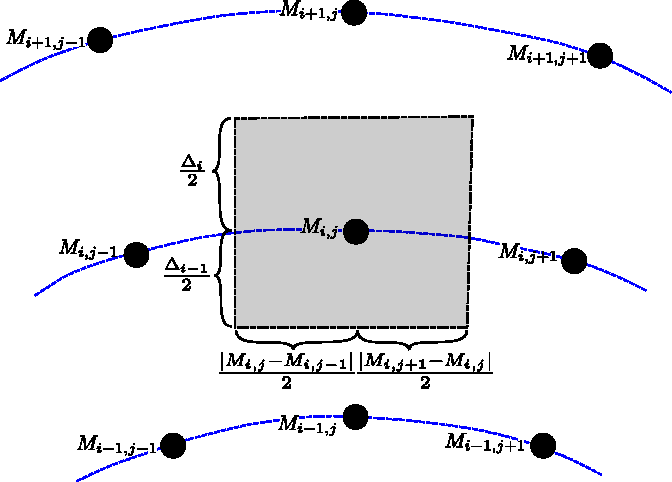
\includegraphics[width=150mm]{fig/weighting.pdf}
\caption{Visualization of the weighting used to compute surface average repulsion $\bar{\lambda}_3$ and surface pseudo-surface area $A_{\mathcal{M}}$. The weight of $M_{i,j}$ is an approximation of the region of $\mathcal{M}$ that is closer to $M_{i,j}$ than any other mesh point (shaded in gray). This is done by computing the area of the rectangle of sides equal to the average of $M_{i,j}$ nearest neighbor distances in the radial direction, as well as along $C_i$.}\label{fig:weighting}
\end{figure}

Note that while the preceding discussion focuses on identification of repelling hyperbolic LCSs, the method is very easily adapted as to instead identify attracting hyperbolic LCSs. This may be done by advecting tracer particles in the time-reversed interval $[t,t_0]$ and thereafter proceeding as discussed.

%%=========================================
%\section{Selecting LCSs from LCS candidate structures}\label{LCS_selection}

%Having determined a set of LCS candidate surfaces by application of the geodesic levelset method, LCS identification is a matter of selecting local repulsion maxima. As will later be discussed in depth, condition 4 (see equation \eqref{eq:ExistenceConditions}) is largely unsuitable for grid based numerical analysis. Note that condition 4 is imposed in order to guarantee that any given point on an LCS is a local repulsion maximum. We may therefore relax condition 4 by instead requiring that the average of $\lambda_3$ on a candidate sirface, hereafter denoted $\overline{\lambda}_3$, must be a local maximum among nearby candidate surfaces. This constitutes the final numerically adapted existence criterion:

%\begin{align}\label{eq:LCS_condition_D}
%\begin{aligned}
%	(D)\quad &\rm{The\ surface\ average\ of\ \lambda_3\ (\overline{\lambda}_3)\ over\ \mathcal{M}(t_0)\ is\ maximal\ among} \\
%	&\rm{local\ surfaces\ \gamma\ satisfying\ \gamma\perp\bm{\xi}_3(\vec{x}_0).}
%\end{aligned}
%\end{align}

%In the interest of simpplicity, the surface repulsion maxima prescribed by condition D were found by direct comparison of $\overline{\lambda_3}$ between neighboring LCS candidate surfaces $\mathcal{M}_{\rm{cand}}$. This was done by defining a set of subdomains $\{U_i\}$, each of which containing one surface repulsion maximum. Specifically, $n_xn_yn_z$ equal rectrangular cuboid subdomains together combrise $U$. The details of this subdomain arrangement are outlined in figure \ref{fig:subdomain_arrangement}.

%\begin{figure}[h!] 
%\centering
%\includegraphics[width=150mm]{fig/subdomain_arrangement.pdf}
%\caption{PLACEHOLDER}
%\label{fig:subdomain_arrangement}
%\end{figure} 

%For each subdomain $U_i$, the $\overline{\lambda_3}$  of the set of LCS candidate surfaces with one or more points contained in $U_i$, are evaluated and compared. The LCS candidate surface associated with the largest $\overline{\lambda_3}$ within the region $U_i$ is then classified as a local repulsion maximum. Having been determined to satisfy all the LCS criteria described in equation [LCS CRITERIA], this LCS candidate has been identified as a hyperbolic repelling LCS. Note that a single LCS candidate spanning several subdomains $U_i$ may act as a repulsion maximum in any number of these subdomains.

%The average $\overline{\lambda}_3$ was determined for each LCS candidate surface by a weighted average of $\lambda_3$ evaluated at all its constituent points. This weighting was chosen to approximate the surface area represented by each sampled point $M_{i,j}$. Specifically, the weighting of $M_{i,j}$, $W_{i,j}$, was computed as 

%\begin{equation}
%W_{i,j} = \frac{\Delta_{i}+\Delta_{i-1}}{2}\frac{\left|M_{i,j}-M_{i,j-1}\right|+\left|M_{i,j+1}-M_{i,j}\right|}{2}.
%\end{equation}

%\noindent That is, the weighting of each manifold point $M_{i,j}$ is defined as to approximate the   region of $\mathcal{M}$ that is closer to $M_{i,j}$ than to any other point in $M$. The physical analog to this weighting is illustrated in figure \ref{fig:weighting}.

%\begin{figure}[h!] 
%\centering
%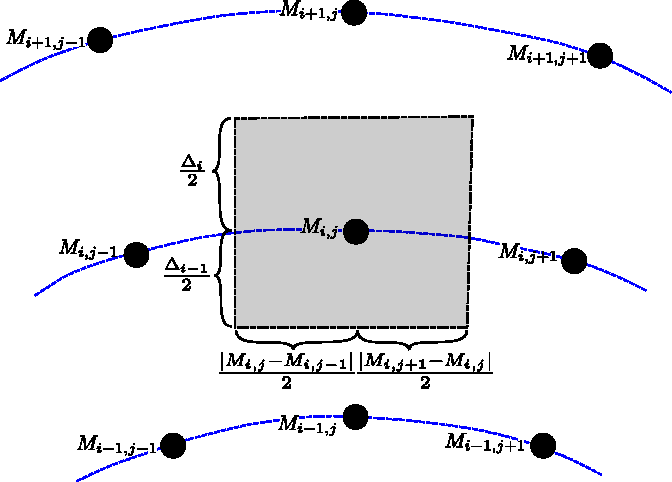
\includegraphics[width=150mm]{fig/weighting.pdf}
%\caption{PLACEHOLDER}
%\label{fig:weighting}
%\end{figure}

%%=========================================
\section{Managing computing time and resource requirements}\label{sec:resource_requirements}

Given that large numbers of manifolds have to be computed from initial positions in order to ensure sufficient coverage of potential LCSs, significant performance gains may be attained from dividing manifold development into separate processes. As each manifold may be computed independent of all other manifolds, no communication is required between the various processes. We disperse the workload among several computation cores by use of MPI. Specifically, this was done by use of the \textit{mpi4py} library in Python. Given the levelset based structure exhibited by the method of geodesic levelsets, it seems highly impractical to parallelize the development of individual manifolds. In particular, the dynamic inter-levelset step length described in section \ref{sec:step_management} and setwise monitoring of numerical noise and self-intersections described in sections \ref{sec:limit_numerical_noise} and \ref{sec:termination_criteria}, would not only require significant overhead in terms of inter-process communication, but also prohibit rapidly progressing point strands from progressing ahead of slower ones.

Like development of manifolds, the flow map and flow map Jacobian ``advection'' is easily parallelizable with minimal needs for inter-process communication. This was done by evenly dispersing the grid particles among all available processing units and subsequently gathering the results after completing each computation. In this way, performance for computing the flow map and flow map Jacobian on large grids may be increased greatly. The potential for speedup is usually limited by the available number of processing units. Representing a much smaller fraction of the total computational load, preparation of manifold initial positions was distributed within a single cluster node by use of the Python \textit{multiprocessing} library. 

The majority of code used in this project was written in Python as to promote accessibility, as well as ease of development. However, as manifolds could consist of tens of thousands of points, each iteratively computed using a Runge-Kutta ODE solver, performance issues may quickly arise. Unsurprisingly, systematic line profiling of the code implementation revealed that time expenditure was largely concentrated in computation of point search trajectories, self-intersection checks, and noise removal.

Most prominent of these, computation of point search trajectories is performed for each new mesh point, possibly requiring a large number of Dormand-Prince method iterations. In order to improve performance, the Dormand-Prince iterative solver, as well as acceptance criteria controls, were reimplemented as C-functions. This was done by use of Cython, an optimizing static compiler that allows for calling C-code from Python, as well as tuning Python code to C performance. Specifically, the Runge-Kutta solver, as well as frequently used functions such as vector normalization and computing Euclidean norms were optimized in C and called directly from Python. This yielded large performance gains.

Similar treatment was given to the self-intersection check and noise reduction implementations, yielding major performance benefits. However, as these modules were comparatively less demanding in terms of workload, the associated absolute performance benefits were moderate.

